\documentclass[a4paper,10pt]{article}
\usepackage[british]{babel}
\usepackage{graphicx}

\newcommand{\FOSDEMday}{Saturday~}
\usepackage{booklet}
\usepackage{talktables}

% The year and edition (2001 was 1st)
% (~ forces a space after the command-text)
\newcommand{\FOSDEMyear}{2015~}
\newcommand{\FOSDEMedition}{15\textsuperscript{th}~}

\begin{document}


% Cover page
%\pagestyle{empty}
\label{cover}
\begin{center}
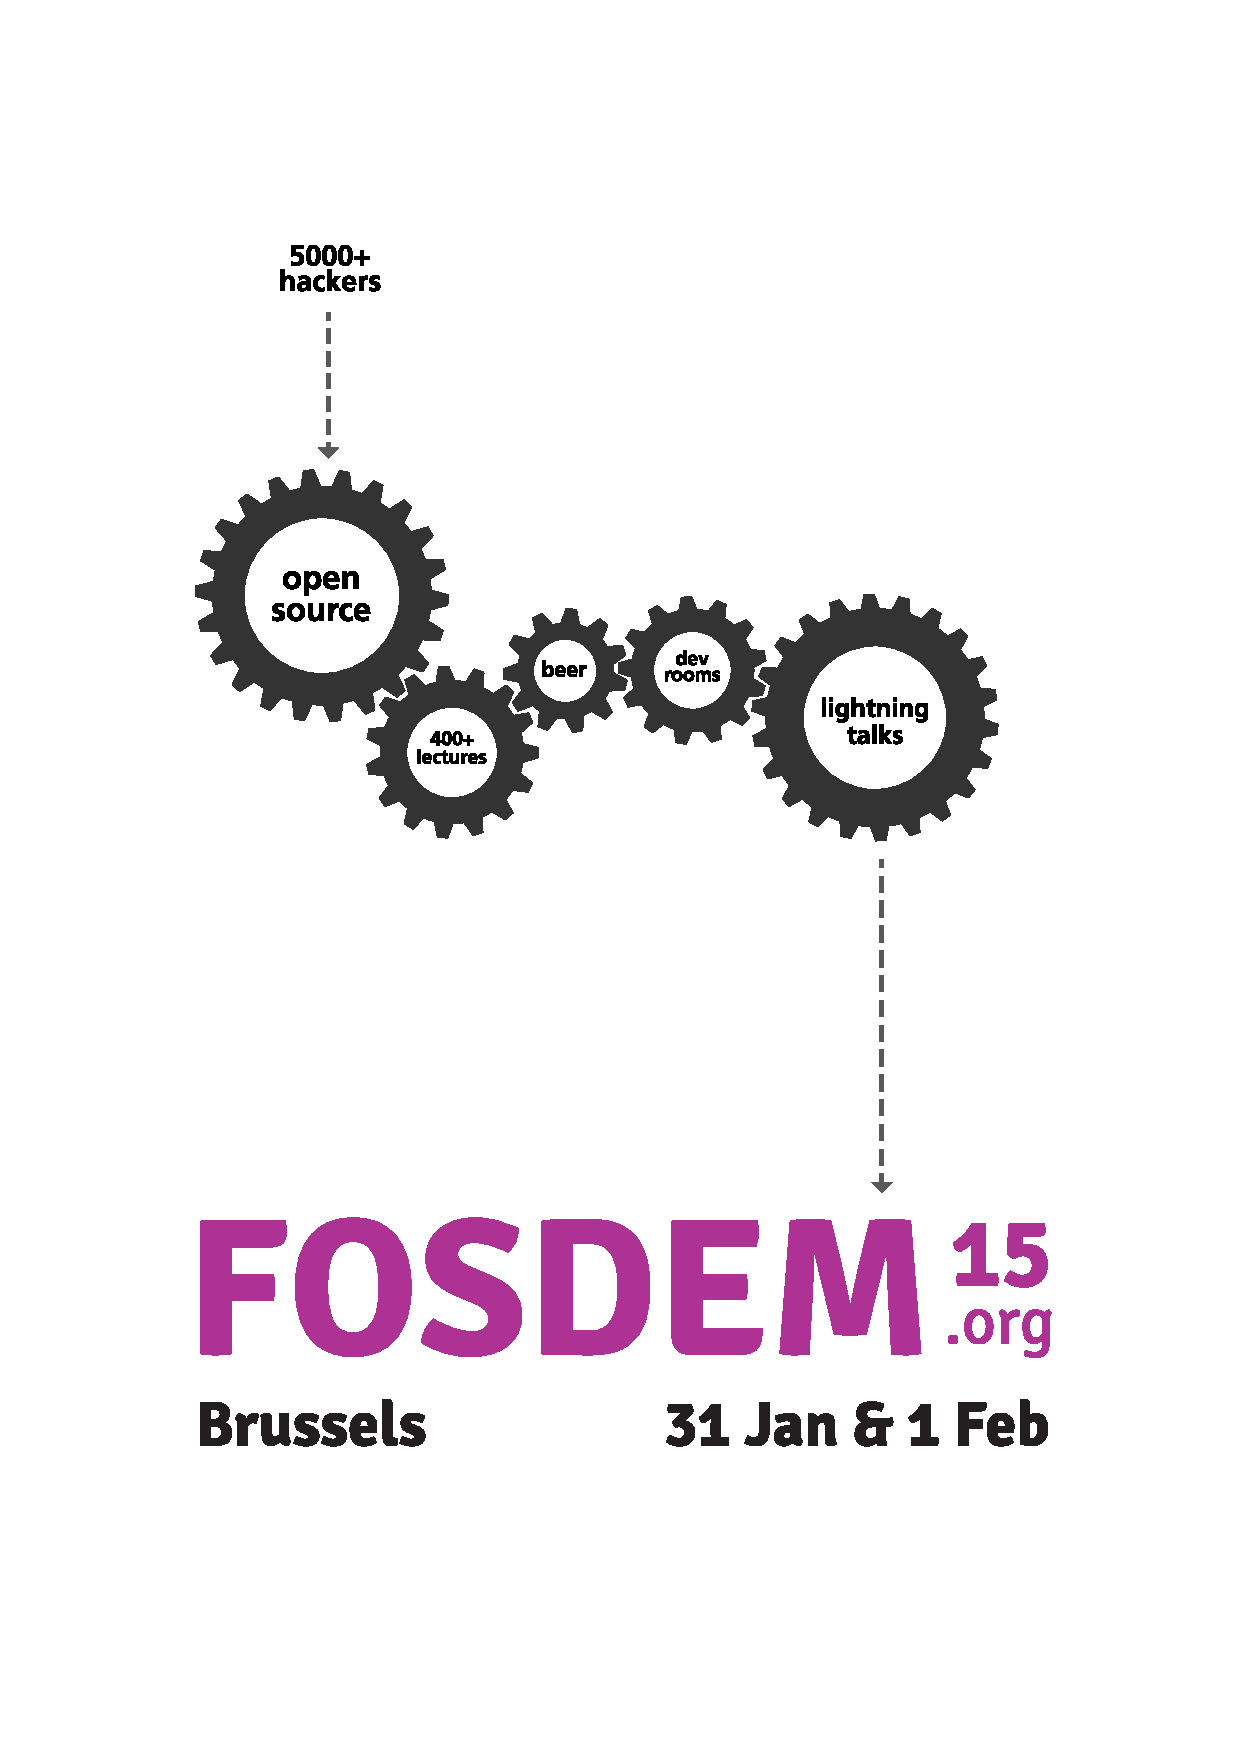
\includegraphics[width=0.6\textwidth]{artwork/flyer_nobg}


{\fontsize{35}{45}\selectfont
\bf

Schedule: Saturday
}

\vfill

% hack: fixed TOC
{\Large
\begin{tabular}{lll}
page 2   & &  Main tracks and lightning talks \\
page 3   & &  Devrooms in AW building \\
page 4-5 & &  Devrooms in H building \\
page 5-6 & &  Devrooms in K building \\
page 6-7 & &  Devrooms in U building \\
\end{tabular}

\vfill

Schedule details and mobile apps on ~\texttt{https://fosdem.org/2015/schedule/}
}

\vfill

\end{center}

Compiled on {\ddmmyyyydate\today} at \currenttime, source code on \texttt{https://github.com/tias/penta\_booklet}

\loadgeometry{default}

% the tables...
{% you may have to tweak these numbers to make all tables fit a page
\fontsize{10.5}{8.09}\selectfont%
\renewcommand{\arraystretch}{0.88}%
%
% generator-hash: c58bb3da9f7693765d6230c3f19a3a05

{\fontsize{9.8}{7.2}\selectfont\renewcommand{\arraystretch}{0.88}% generator-hash: 7f669240362efade63f684f585863210

\pagebreak\begin{talktable}{3}
 & \HeaderTitle{Main tracks} & \HeaderTitle{Main tracks} & \HeaderTitle{Lightning talks}\\ 
 & \HeaderSubtitle{J.Janson} & \HeaderSubtitle{K.1.105 (La Fontaine)} & \HeaderSubtitle{H.2215 (Ferrer)}\\ \hhline{*{4}-} 
\raisebox{-0.33ex}{\small\bf ! 09:30 !} & \CellBG &  & \\ \hhline{>{\arrayrulecolor{black}}->{\arrayrulecolor{gray!20}}-~~} 
 & \CellBG &  & \\ \hhline{>{\arrayrulecolor{black}}->{\arrayrulecolor{gray!20}}-~~} 
 & \CellBG &  & \\ \hhline{>{\arrayrulecolor{black}}->{\arrayrulecolor{gray!20}}-~~} 
\raisebox{-0.33ex}{\small 09:45} & \CellBG &  & \\ \hhline{>{\arrayrulecolor{black}}->{\arrayrulecolor{gray!20}}-~~} 
 & \CellTalk{5}{Welcome to FOSDEM 2015}{FOSDEM Staff}
 &  & \\ \hhline{>{\arrayrulecolor{black}}->{\arrayrulecolor{black}}-~~} 
 &  &  & \\ \hhline{>{\arrayrulecolor{black}}->{\arrayrulecolor{black}}-~~} 
\raisebox{-0.33ex}{\small\bf 10:00} & \CellBG &  & \\ \hhline{>{\arrayrulecolor{black}}->{\arrayrulecolor{gray!20}}-~~} 
 & \CellBG &  & \\ \hhline{>{\arrayrulecolor{black}}->{\arrayrulecolor{gray!20}}-~~} 
 & \CellBG &  & \\ \hhline{>{\arrayrulecolor{black}}->{\arrayrulecolor{gray!20}}-~~} 
\raisebox{-0.33ex}{\small 10:15} & \CellBG &  & \\ \hhline{>{\arrayrulecolor{black}}->{\arrayrulecolor{gray!20}}-~~} 
 & \CellBG &  & \\ \hhline{>{\arrayrulecolor{black}}->{\arrayrulecolor{gray!20}}-~~} 
 & \CellBG &  & \\ \hhline{>{\arrayrulecolor{black}}->{\arrayrulecolor{gray!20}}-~~} 
\raisebox{-0.33ex}{\small 10:30} & \CellBG &  & \\ \hhline{>{\arrayrulecolor{black}}->{\arrayrulecolor{gray!20}}-~~} 
 & \CellBG &  & \\ \hhline{>{\arrayrulecolor{black}}->{\arrayrulecolor{gray!20}}-~~} 
 & \CellBG &  & \\ \hhline{>{\arrayrulecolor{black}}->{\arrayrulecolor{gray!20}}-~~} 
\raisebox{-0.33ex}{\small 10:45} & \CellTalk{10}{Identity Crisis: Are we who we say we are?}{Karen Sandler}
 &  & \\ \hhline{>{\arrayrulecolor{black}}->{\arrayrulecolor{black}}-~~} 
 &  &  & \\ \hhline{>{\arrayrulecolor{black}}-~~~} 
 &  &  & \\ \hhline{>{\arrayrulecolor{black}}->{\arrayrulecolor{black}}-~~} 
\raisebox{-0.33ex}{\small\bf 11:00} & \CellBG &  & \\ \hhline{>{\arrayrulecolor{black}}->{\arrayrulecolor{gray!20}}-~~} 
 & \CellBG &  & \\ \hhline{>{\arrayrulecolor{black}}->{\arrayrulecolor{gray!20}}-~~} 
 & \CellBG &  & \\ \hhline{>{\arrayrulecolor{black}}->{\arrayrulecolor{gray!20}}-~~} 
\raisebox{-0.33ex}{\small 11:15} & \CellBG &  & \\ \hhline{>{\arrayrulecolor{black}}->{\arrayrulecolor{gray!20}}-~~} 
 & \CellBG &  & \\ \hhline{>{\arrayrulecolor{black}}->{\arrayrulecolor{gray!20}}-~~} 
 & \CellBG &  & \\ \hhline{>{\arrayrulecolor{black}}->{\arrayrulecolor{gray!20}}-~~} 
\raisebox{-0.33ex}{\small 11:30} & \CellBG &  & \\ \hhline{>{\arrayrulecolor{black}}->{\arrayrulecolor{gray!20}}-~~} 
 & \CellBG &  & \\ \hhline{>{\arrayrulecolor{black}}->{\arrayrulecolor{gray!20}}-~~} 
 & \CellBG &  & \\ \hhline{>{\arrayrulecolor{black}}->{\arrayrulecolor{gray!20}}-~~} 
\raisebox{-0.33ex}{\small 11:45} & \CellTalk{10}{What is wrong with Operating Systems}{Antti Kantee}
 &  & \\ \hhline{>{\arrayrulecolor{black}}->{\arrayrulecolor{black}}-~~} 
 &  &  & \\ \hhline{>{\arrayrulecolor{black}}-~~~} 
 &  &  & \\ \hhline{>{\arrayrulecolor{black}}->{\arrayrulecolor{black}}->{\arrayrulecolor{black}}-~} 
\raisebox{-0.33ex}{\small\bf 12:00} & \CellBG & \CellBG & \\ \hhline{>{\arrayrulecolor{black}}->{\arrayrulecolor{gray!20}}->{\arrayrulecolor{gray!20}}-~} 
 & \CellBG & \CellBG & \\ \hhline{>{\arrayrulecolor{black}}->{\arrayrulecolor{gray!20}}->{\arrayrulecolor{gray!20}}-~} 
 & \CellBG & \CellBG & \\ \hhline{>{\arrayrulecolor{black}}->{\arrayrulecolor{gray!20}}->{\arrayrulecolor{gray!20}}-~} 
\raisebox{-0.33ex}{\small 12:15} & \CellBG & \CellBG & \\ \hhline{>{\arrayrulecolor{black}}->{\arrayrulecolor{gray!20}}->{\arrayrulecolor{gray!20}}-~} 
 & \CellBG & \CellBG & \\ \hhline{>{\arrayrulecolor{black}}->{\arrayrulecolor{gray!20}}->{\arrayrulecolor{gray!20}}-~} 
 & \CellBG & \CellBG & \\ \hhline{>{\arrayrulecolor{black}}->{\arrayrulecolor{gray!20}}->{\arrayrulecolor{gray!20}}-~} 
\raisebox{-0.33ex}{\small 12:30} & \CellBG & \CellBG & \\ \hhline{>{\arrayrulecolor{black}}->{\arrayrulecolor{gray!20}}->{\arrayrulecolor{gray!20}}-~} 
 & \CellBG & \CellBG & \\ \hhline{>{\arrayrulecolor{black}}->{\arrayrulecolor{gray!20}}->{\arrayrulecolor{gray!20}}-~} 
 & \CellBG & \CellBG & \\ \hhline{>{\arrayrulecolor{black}}->{\arrayrulecolor{gray!20}}->{\arrayrulecolor{gray!20}}-~} 
\raisebox{-0.33ex}{\small 12:45} & \CellTalk{10}{Automating Attribution}{Jonas \"{O}berg}
 & \CellTalk{10}{A GPS watch made of free software and hardware}{Federico Vaga, Matthieu Cattin}
 & \\ \hhline{>{\arrayrulecolor{black}}->{\arrayrulecolor{black}}->{\arrayrulecolor{black}}-~} 
 &  &  & \\ \hhline{>{\arrayrulecolor{black}}-~~>{\arrayrulecolor{black}}-} 
 &  &  & \CellTalkSingleSmall{1}{Lightning Talks Welcome}{}
\\ \hhline{>{\arrayrulecolor{black}}->{\arrayrulecolor{black}}->{\arrayrulecolor{black}}->{\arrayrulecolor{black}}-} 
\raisebox{-0.33ex}{\small\bf 13:00} & \CellBG & \CellBG & \CellBG\\ \hhline{>{\arrayrulecolor{black}}->{\arrayrulecolor{gray!20}}->{\arrayrulecolor{gray!20}}->{\arrayrulecolor{gray!20}}-} 
 & \CellBG & \CellBG & \CellBG\\ \hhline{>{\arrayrulecolor{black}}->{\arrayrulecolor{gray!20}}->{\arrayrulecolor{gray!20}}->{\arrayrulecolor{gray!20}}-} 
 & \CellBG & \CellBG & \CellTalkCompact{3}{Developing FOSDEM Companion}{Christophe Beyls}
\\ \hhline{>{\arrayrulecolor{black}}->{\arrayrulecolor{gray!20}}->{\arrayrulecolor{gray!20}}->{\arrayrulecolor{black}}-} 
\raisebox{-0.33ex}{\small 13:15} & \CellBG & \CellBG & \\ \hhline{>{\arrayrulecolor{black}}->{\arrayrulecolor{gray!20}}->{\arrayrulecolor{gray!20}}->{\arrayrulecolor{black}}-} 
 & \CellBG & \CellBG & \CellBG\\ \hhline{>{\arrayrulecolor{black}}->{\arrayrulecolor{gray!20}}->{\arrayrulecolor{gray!20}}->{\arrayrulecolor{gray!20}}-} 
 & \CellBG & \CellBG & \CellBG\\ \hhline{>{\arrayrulecolor{black}}->{\arrayrulecolor{gray!20}}->{\arrayrulecolor{gray!20}}->{\arrayrulecolor{gray!20}}-} 
\raisebox{-0.33ex}{\small 13:30} & \CellBG & \CellBG & \CellTalkCompact{3}{Ultra -- Smallest. Web server. Evar.}{Steven Goodwin}
\\ \hhline{>{\arrayrulecolor{black}}->{\arrayrulecolor{gray!20}}->{\arrayrulecolor{gray!20}}->{\arrayrulecolor{black}}-} 
 & \CellBG & \CellBG & \\ \hhline{>{\arrayrulecolor{black}}->{\arrayrulecolor{gray!20}}->{\arrayrulecolor{gray!20}}->{\arrayrulecolor{black}}-} 
 & \CellBG & \CellBG & \CellBG\\ \hhline{>{\arrayrulecolor{black}}->{\arrayrulecolor{gray!20}}->{\arrayrulecolor{gray!20}}->{\arrayrulecolor{gray!20}}-} 
\raisebox{-0.33ex}{\small 13:45} & \CellTalk{10}{A new version of Firefox is available}{Sylvestre Ledru, Lukas Blakk}
 & \CellTalk{10}{lowRISC}{Alex Bradbury}
 & \CellBG\\ \hhline{>{\arrayrulecolor{black}}->{\arrayrulecolor{black}}->{\arrayrulecolor{black}}->{\arrayrulecolor{gray!20}}-} 
 &  &  & \CellTalkCompact{3}{How adblockers work}{Sebastian Noack}
\\ \hhline{>{\arrayrulecolor{black}}-~~>{\arrayrulecolor{black}}-} 
 &  &  & \\ \hhline{>{\arrayrulecolor{black}}->{\arrayrulecolor{black}}->{\arrayrulecolor{black}}->{\arrayrulecolor{black}}-} 
\raisebox{-0.33ex}{\small\bf 14:00} & \CellBG & \CellBG & \CellBG\\ \hhline{>{\arrayrulecolor{black}}->{\arrayrulecolor{gray!20}}->{\arrayrulecolor{gray!20}}->{\arrayrulecolor{gray!20}}-} 
 & \CellBG & \CellBG & \CellBG\\ \hhline{>{\arrayrulecolor{black}}->{\arrayrulecolor{gray!20}}->{\arrayrulecolor{gray!20}}->{\arrayrulecolor{gray!20}}-} 
 & \CellBG & \CellBG & \CellTalkCompact{3}{A Whirlwind Introduction to OpenUI5}{DJ Adams}
\\ \hhline{>{\arrayrulecolor{black}}->{\arrayrulecolor{gray!20}}->{\arrayrulecolor{gray!20}}->{\arrayrulecolor{black}}-} 
\raisebox{-0.33ex}{\small 14:15} & \CellBG & \CellBG & \\ \hhline{>{\arrayrulecolor{black}}->{\arrayrulecolor{gray!20}}->{\arrayrulecolor{gray!20}}->{\arrayrulecolor{black}}-} 
 & \CellBG & \CellBG & \CellBG\\ \hhline{>{\arrayrulecolor{black}}->{\arrayrulecolor{gray!20}}->{\arrayrulecolor{gray!20}}->{\arrayrulecolor{gray!20}}-} 
 & \CellBG & \CellBG & \CellBG\\ \hhline{>{\arrayrulecolor{black}}->{\arrayrulecolor{gray!20}}->{\arrayrulecolor{gray!20}}->{\arrayrulecolor{gray!20}}-} 
\raisebox{-0.33ex}{\small 14:30} & \CellBG & \CellBG & \CellTalkCompact{3}{All about Hack in 15 minutes}{Tobias Nyholm}
\\ \hhline{>{\arrayrulecolor{black}}->{\arrayrulecolor{gray!20}}->{\arrayrulecolor{gray!20}}->{\arrayrulecolor{black}}-} 
 & \CellBG & \CellBG & \\ \hhline{>{\arrayrulecolor{black}}->{\arrayrulecolor{gray!20}}->{\arrayrulecolor{gray!20}}->{\arrayrulecolor{black}}-} 
 & \CellBG & \CellBG & \CellBG\\ \hhline{>{\arrayrulecolor{black}}->{\arrayrulecolor{gray!20}}->{\arrayrulecolor{gray!20}}->{\arrayrulecolor{gray!20}}-} 
\raisebox{-0.33ex}{\small 14:45} & \CellTalk{10}{Building High-Performance Language Implementations With Low Effort}{Stefan Marr}
 & \CellTalk{10}{BERI}{Jonathan Woodruff}
 & \CellBG\\ \hhline{>{\arrayrulecolor{black}}->{\arrayrulecolor{black}}->{\arrayrulecolor{black}}->{\arrayrulecolor{gray!20}}-} 
 &  &  & \CellTalkCompact{3}{CockroachDB}{Tobias Schottdorf}
\\ \hhline{>{\arrayrulecolor{black}}-~~>{\arrayrulecolor{black}}-} 
 &  &  & \\ \hhline{>{\arrayrulecolor{black}}->{\arrayrulecolor{black}}->{\arrayrulecolor{black}}->{\arrayrulecolor{black}}-} 
\raisebox{-0.33ex}{\small\bf 15:00} & \CellBG & \CellBG & \CellBG\\ \hhline{>{\arrayrulecolor{black}}->{\arrayrulecolor{gray!20}}->{\arrayrulecolor{gray!20}}->{\arrayrulecolor{gray!20}}-} 
 & \CellBG & \CellBG & \CellBG\\ \hhline{>{\arrayrulecolor{black}}->{\arrayrulecolor{gray!20}}->{\arrayrulecolor{gray!20}}->{\arrayrulecolor{gray!20}}-} 
 & \CellBG & \CellBG & \CellTalkCompact{3}{GCompris goes Qt Quick with the help of KDE}{Bruno Coudoin}
\\ \hhline{>{\arrayrulecolor{black}}->{\arrayrulecolor{gray!20}}->{\arrayrulecolor{gray!20}}->{\arrayrulecolor{black}}-} 
\raisebox{-0.33ex}{\small 15:15} & \CellBG & \CellBG & \\ \hhline{>{\arrayrulecolor{black}}->{\arrayrulecolor{gray!20}}->{\arrayrulecolor{gray!20}}->{\arrayrulecolor{black}}-} 
 & \CellBG & \CellBG & \CellBG\\ \hhline{>{\arrayrulecolor{black}}->{\arrayrulecolor{gray!20}}->{\arrayrulecolor{gray!20}}->{\arrayrulecolor{gray!20}}-} 
 & \CellBG & \CellBG & \CellBG\\ \hhline{>{\arrayrulecolor{black}}->{\arrayrulecolor{gray!20}}->{\arrayrulecolor{gray!20}}->{\arrayrulecolor{gray!20}}-} 
\raisebox{-0.33ex}{\small 15:30} & \CellBG & \CellBG & \CellTalkCompact{3}{Requirements Bazaar}{Istv\`{a}n Koren}
\\ \hhline{>{\arrayrulecolor{black}}->{\arrayrulecolor{gray!20}}->{\arrayrulecolor{gray!20}}->{\arrayrulecolor{black}}-} 
 & \CellBG & \CellBG & \\ \hhline{>{\arrayrulecolor{black}}->{\arrayrulecolor{gray!20}}->{\arrayrulecolor{gray!20}}->{\arrayrulecolor{black}}-} 
 & \CellBG & \CellBG & \CellBG\\ \hhline{>{\arrayrulecolor{black}}->{\arrayrulecolor{gray!20}}->{\arrayrulecolor{gray!20}}->{\arrayrulecolor{gray!20}}-} 
\raisebox{-0.33ex}{\small 15:45} & \CellTalk{10}{IgProf}{Giulio Eulisse}
 & \CellTalk{10}{FreeCAD}{Yorik van Havre}
 & \CellBG\\ \hhline{>{\arrayrulecolor{black}}->{\arrayrulecolor{black}}->{\arrayrulecolor{black}}->{\arrayrulecolor{gray!20}}-} 
 &  &  & \CellTalkCompact{3}{Scalable Video Conf. with Jitsi Videobridge}{Emil Ivov}
\\ \hhline{>{\arrayrulecolor{black}}-~~>{\arrayrulecolor{black}}-} 
 &  &  & \\ \hhline{>{\arrayrulecolor{black}}->{\arrayrulecolor{black}}->{\arrayrulecolor{black}}->{\arrayrulecolor{black}}-} 
\raisebox{-0.33ex}{\small\bf 16:00} & \CellBG & \CellBG & \CellBG\\ \hhline{>{\arrayrulecolor{black}}->{\arrayrulecolor{gray!20}}->{\arrayrulecolor{gray!20}}->{\arrayrulecolor{gray!20}}-} 
 & \CellBG & \CellBG & \CellBG\\ \hhline{>{\arrayrulecolor{black}}->{\arrayrulecolor{gray!20}}->{\arrayrulecolor{gray!20}}->{\arrayrulecolor{gray!20}}-} 
 & \CellBG & \CellBG & \CellTalkCompact{3}{XMPP and Android}{Florian Schmaus}
\\ \hhline{>{\arrayrulecolor{black}}->{\arrayrulecolor{gray!20}}->{\arrayrulecolor{gray!20}}->{\arrayrulecolor{black}}-} 
\raisebox{-0.33ex}{\small 16:15} & \CellBG & \CellBG & \\ \hhline{>{\arrayrulecolor{black}}->{\arrayrulecolor{gray!20}}->{\arrayrulecolor{gray!20}}->{\arrayrulecolor{black}}-} 
 & \CellBG & \CellBG & \CellBG\\ \hhline{>{\arrayrulecolor{black}}->{\arrayrulecolor{gray!20}}->{\arrayrulecolor{gray!20}}->{\arrayrulecolor{gray!20}}-} 
 & \CellBG & \CellBG & \CellBG\\ \hhline{>{\arrayrulecolor{black}}->{\arrayrulecolor{gray!20}}->{\arrayrulecolor{gray!20}}->{\arrayrulecolor{gray!20}}-} 
\raisebox{-0.33ex}{\small 16:30} & \CellBG & \CellBG & \CellTalkInline{3}{Matrix.org -- a new open standard for distributed, \ldots}{Oddvar Lovaas, Matthew Hodgson}
\\ \hhline{>{\arrayrulecolor{black}}->{\arrayrulecolor{gray!20}}->{\arrayrulecolor{gray!20}}->{\arrayrulecolor{black}}-} 
 & \CellBG & \CellBG & \\ \hhline{>{\arrayrulecolor{black}}->{\arrayrulecolor{gray!20}}->{\arrayrulecolor{gray!20}}->{\arrayrulecolor{black}}-} 
 & \CellBG & \CellBG & \CellBG\\ \hhline{>{\arrayrulecolor{black}}->{\arrayrulecolor{gray!20}}->{\arrayrulecolor{gray!20}}->{\arrayrulecolor{gray!20}}-} 
\raisebox{-0.33ex}{\small 16:45} & \CellTalk{10}{Superoptimization}{James Pallister}
 & \CellTalk{10}{Stretching out for trustworthy reproducible builds}{Holger Levsen}
 & \CellBG\\ \hhline{>{\arrayrulecolor{black}}->{\arrayrulecolor{black}}->{\arrayrulecolor{black}}->{\arrayrulecolor{gray!20}}-} 
 &  &  & \CellTalkInline{3}{Yatta: A Real-Time Framework for Peer-to-peer Group Editing ...}{Petru Nicolaescu, Kevin Jahns}
\\ \hhline{>{\arrayrulecolor{black}}-~~>{\arrayrulecolor{black}}-} 
 &  &  & \\ \hhline{>{\arrayrulecolor{black}}->{\arrayrulecolor{black}}-~>{\arrayrulecolor{black}}-} 
\raisebox{-0.33ex}{\small\bf 17:00} & \CellBG &  & \CellBG\\ \hhline{>{\arrayrulecolor{black}}->{\arrayrulecolor{gray!20}}-~>{\arrayrulecolor{gray!20}}-} 
 & \CellBG &  & \CellBG\\ \hhline{>{\arrayrulecolor{black}}->{\arrayrulecolor{gray!20}}-~>{\arrayrulecolor{gray!20}}-} 
 & \CellBG &  & \CellTalkCompact{3}{Building an Open Source VoIP hardware phone}{Sa\'{u}l Ibarra Corretg\'{e}}
\\ \hhline{>{\arrayrulecolor{black}}->{\arrayrulecolor{gray!20}}-~>{\arrayrulecolor{black}}-} 
\raisebox{-0.33ex}{\small 17:15} & \CellBG &  & \\ \hhline{>{\arrayrulecolor{black}}->{\arrayrulecolor{gray!20}}-~>{\arrayrulecolor{black}}-} 
 & \CellBG &  & \CellBG\\ \hhline{>{\arrayrulecolor{black}}->{\arrayrulecolor{gray!20}}-~>{\arrayrulecolor{gray!20}}-} 
 & \CellBG &  & \CellBG\\ \hhline{>{\arrayrulecolor{black}}->{\arrayrulecolor{gray!20}}-~>{\arrayrulecolor{gray!20}}-} 
\raisebox{-0.33ex}{\small 17:30} & \CellBG &  & \CellTalkCompact{3}{codebender: Arduino programing, online}{Vasileios Georgitzikis}
\\ \hhline{>{\arrayrulecolor{black}}->{\arrayrulecolor{gray!20}}-~>{\arrayrulecolor{black}}-} 
 & \CellBG &  & \\ \hhline{>{\arrayrulecolor{black}}->{\arrayrulecolor{gray!20}}-~>{\arrayrulecolor{black}}-} 
 & \CellBG &  & \CellBG\\ \hhline{>{\arrayrulecolor{black}}->{\arrayrulecolor{gray!20}}-~>{\arrayrulecolor{gray!20}}-} 
\raisebox{-0.33ex}{\small 17:45} & \CellTalk{10}{Ubiquitous Performance Analysis and System Introspection}{Lukas Berk}
 &  & \CellBG\\ \hhline{>{\arrayrulecolor{black}}->{\arrayrulecolor{black}}-~>{\arrayrulecolor{gray!20}}-} 
 &  &  & \CellTalkInline{3}{Rizzly: Event Driven Microcontroller Programming}{Urs F\"{a}ssler}
\\ \hhline{>{\arrayrulecolor{black}}-~~>{\arrayrulecolor{black}}-} 
 &  &  & \\ \hhline{>{\arrayrulecolor{black}}-~~>{\arrayrulecolor{black}}-} 
\raisebox{-0.33ex}{\small\bf 18:00} &  &  & \CellBG\\ \hhline{>{\arrayrulecolor{black}}-~~>{\arrayrulecolor{gray!20}}-} 
 &  &  & \CellBG\\ \hhline{>{\arrayrulecolor{black}}-~~>{\arrayrulecolor{gray!20}}-} 
 &  &  & \CellTalkCompact{3}{Crazyflie Nano Quadcopter}{Frederic Gurr}
\\ \hhline{>{\arrayrulecolor{black}}-~~>{\arrayrulecolor{black}}-} 
\raisebox{-0.33ex}{\small 18:15} &  &  & \\ \hhline{>{\arrayrulecolor{black}}-~~>{\arrayrulecolor{black}}-} 
 &  &  & \CellBG\\ \hhline{>{\arrayrulecolor{black}}-~~>{\arrayrulecolor{gray!20}}-} 
 &  &  & \CellBG\\ \hhline{>{\arrayrulecolor{black}}-~~>{\arrayrulecolor{gray!20}}-} 
\raisebox{-0.33ex}{\small 18:30} &  &  & \CellTalkCompact{3}{LLVMLinux}{Behan Webster}
\\ \hhline{>{\arrayrulecolor{black}}-~~>{\arrayrulecolor{black}}-} 
 &  &  & \\ \hhline{>{\arrayrulecolor{black}}-~~>{\arrayrulecolor{black}}-} 
 &  &  & \CellBG\\ \hhline{>{\arrayrulecolor{black}}-~~>{\arrayrulecolor{gray!20}}-} 
\raisebox{-0.33ex}{\small 18:45} &  &  & \CellBG\\ \hhline{>{\arrayrulecolor{black}}-~~>{\arrayrulecolor{gray!20}}-} 
 &  &  & \CellTalkCompact{3}{Pretty-printing kernel data structures}{Daniel Lovasko}
\\ \hhline{>{\arrayrulecolor{black}}-~~>{\arrayrulecolor{black}}-} 
\end{talktable}%
}
% generator-hash: 54260721aa8dff7876ee5c325b3feac4

\pagebreak\begin{talktable}{4}
 & \HeaderTitle{Valgrind} & \HeaderTitle{BSD} & \HeaderTitle{Ada} & \HeaderTitle{Graph processing}\\ 
 & \HeaderSubtitle{AW.120} & \HeaderSubtitle{AW.121} & \HeaderSubtitle{AW.124} & \HeaderSubtitle{AW.125}\\ \hhline{*{5}-} 
\raisebox{-0.33ex}{\small 10:30} & \CellBG & \CellBG & \CellBG & \CellBG\\ \hhline{>{\arrayrulecolor{black}}->{\arrayrulecolor{gray!20}}->{\arrayrulecolor{gray!20}}->{\arrayrulecolor{gray!20}}->{\arrayrulecolor{gray!20}}-} 
 & \CellBG & \CellBG & \CellBG & \CellBG\\ \hhline{>{\arrayrulecolor{black}}->{\arrayrulecolor{gray!20}}->{\arrayrulecolor{gray!20}}->{\arrayrulecolor{gray!20}}->{\arrayrulecolor{gray!20}}-} 
 & \CellBG & \CellBG & \CellBG & \CellTalkCompact{3}{Welcome to the GraphDevroom}{Achim Friedland, Pere Urbon-Bayes}
\\ \hhline{>{\arrayrulecolor{black}}->{\arrayrulecolor{gray!20}}->{\arrayrulecolor{gray!20}}->{\arrayrulecolor{gray!20}}->{\arrayrulecolor{black}}-} 
\raisebox{-0.33ex}{\small 10:45} & \CellBG & \CellBG & \CellBG & \CellBG\\ \hhline{>{\arrayrulecolor{black}}->{\arrayrulecolor{gray!20}}->{\arrayrulecolor{gray!20}}->{\arrayrulecolor{gray!20}}->{\arrayrulecolor{gray!20}}-} 
 & \CellBG & \CellBG & \CellBG & \CellBG\\ \hhline{>{\arrayrulecolor{black}}->{\arrayrulecolor{gray!20}}->{\arrayrulecolor{gray!20}}->{\arrayrulecolor{gray!20}}->{\arrayrulecolor{gray!20}}-} 
 & \CellBG & \CellBG & \CellTalk{6}{Arrival \& Informal Discussions}{}
 & \CellBG\\ \hhline{>{\arrayrulecolor{black}}->{\arrayrulecolor{gray!20}}->{\arrayrulecolor{gray!20}}->{\arrayrulecolor{black}}->{\arrayrulecolor{gray!20}}-} 
\raisebox{-0.33ex}{\small\bf 11:00} & \CellBG & \CellBG & \CellTalkSingleSmall{1}{Welcome}{}
 & \CellBG\\ \hhline{>{\arrayrulecolor{black}}->{\arrayrulecolor{gray!20}}->{\arrayrulecolor{gray!20}}->{\arrayrulecolor{black}}->{\arrayrulecolor{gray!20}}-} 
 & \CellBG & \CellBG & \CellBG & \CellBG\\ \hhline{>{\arrayrulecolor{black}}->{\arrayrulecolor{gray!20}}->{\arrayrulecolor{gray!20}}->{\arrayrulecolor{gray!20}}->{\arrayrulecolor{gray!20}}-} 
 & \CellBG & \CellBG & \CellBG & \CellBG\\ \hhline{>{\arrayrulecolor{black}}->{\arrayrulecolor{gray!20}}->{\arrayrulecolor{gray!20}}->{\arrayrulecolor{gray!20}}->{\arrayrulecolor{gray!20}}-} 
\raisebox{-0.33ex}{\small 11:15} & \CellTalk{10}{Valgrind Integration in the Eclipse IDE}{Lukas Berk}
 & \CellBG & \CellBG & \CellBG\\ \hhline{>{\arrayrulecolor{black}}->{\arrayrulecolor{black}}->{\arrayrulecolor{gray!20}}->{\arrayrulecolor{gray!20}}->{\arrayrulecolor{gray!20}}-} 
 &  & \CellBG & \CellBG & \CellBG\\ \hhline{>{\arrayrulecolor{black}}-~>{\arrayrulecolor{gray!20}}->{\arrayrulecolor{gray!20}}->{\arrayrulecolor{gray!20}}-} 
 &  & \CellTalk{12}{EdgeBSD: Status report}{Pierre Pronchery}
 & \CellBG & \CellTalk{9}{Large-scale graph processing with Apache Flink}{Vasia Kalavri}
\\ \hhline{>{\arrayrulecolor{black}}->{\arrayrulecolor{black}}->{\arrayrulecolor{black}}->{\arrayrulecolor{gray!20}}->{\arrayrulecolor{black}}-} 
\raisebox{-0.33ex}{\small 11:30} & \CellBG &  & \CellBG & \CellBG\\ \hhline{>{\arrayrulecolor{black}}->{\arrayrulecolor{gray!20}}-~>{\arrayrulecolor{gray!20}}->{\arrayrulecolor{gray!20}}-} 
 & \CellBG &  & \CellBG & \CellBG\\ \hhline{>{\arrayrulecolor{black}}->{\arrayrulecolor{gray!20}}-~>{\arrayrulecolor{gray!20}}->{\arrayrulecolor{gray!20}}-} 
 & \CellBG &  & \CellBG & \CellBG\\ \hhline{>{\arrayrulecolor{black}}->{\arrayrulecolor{gray!20}}->{\arrayrulecolor{black}}->{\arrayrulecolor{gray!20}}->{\arrayrulecolor{gray!20}}-} 
\raisebox{-0.33ex}{\small 11:45} & \CellBG & \CellBG & \CellBG & \CellBG\\ \hhline{>{\arrayrulecolor{black}}->{\arrayrulecolor{gray!20}}->{\arrayrulecolor{gray!20}}->{\arrayrulecolor{gray!20}}->{\arrayrulecolor{gray!20}}-} 
 & \CellBG & \CellBG & \CellTalk{10}{Ada, an Introduction}{J\'{e}r\'{e}my Rosen}
 & \CellBG\\ \hhline{>{\arrayrulecolor{black}}->{\arrayrulecolor{gray!20}}->{\arrayrulecolor{gray!20}}->{\arrayrulecolor{black}}->{\arrayrulecolor{gray!20}}-} 
 & \CellBG & \CellBG &  & \CellBG\\ \hhline{>{\arrayrulecolor{black}}->{\arrayrulecolor{gray!20}}->{\arrayrulecolor{gray!20}}->{\arrayrulecolor{black}}->{\arrayrulecolor{gray!20}}-} 
\raisebox{-0.33ex}{\small\bf 12:00} & \CellBG & \CellBG & \CellBG & \CellBG\\ \hhline{>{\arrayrulecolor{black}}->{\arrayrulecolor{gray!20}}->{\arrayrulecolor{gray!20}}->{\arrayrulecolor{gray!20}}->{\arrayrulecolor{gray!20}}-} 
 & \CellBG & \CellBG & \CellBG & \CellBG\\ \hhline{>{\arrayrulecolor{black}}->{\arrayrulecolor{gray!20}}->{\arrayrulecolor{gray!20}}->{\arrayrulecolor{gray!20}}->{\arrayrulecolor{gray!20}}-} 
 & \CellBG & \CellBG & \CellBG & \CellBG\\ \hhline{>{\arrayrulecolor{black}}->{\arrayrulecolor{gray!20}}->{\arrayrulecolor{gray!20}}->{\arrayrulecolor{gray!20}}->{\arrayrulecolor{gray!20}}-} 
\raisebox{-0.33ex}{\small 12:15} & \CellTalk{10}{Tuning Valgrind for your Workload}{Philippe Waroquiers}
 & \CellBG & \CellBG & \CellBG\\ \hhline{>{\arrayrulecolor{black}}->{\arrayrulecolor{black}}->{\arrayrulecolor{gray!20}}->{\arrayrulecolor{gray!20}}->{\arrayrulecolor{gray!20}}-} 
 &  & \CellBG & \CellBG & \CellBG\\ \hhline{>{\arrayrulecolor{black}}-~>{\arrayrulecolor{gray!20}}->{\arrayrulecolor{gray!20}}->{\arrayrulecolor{gray!20}}-} 
 &  & \CellTalk{9}{Enlightenment, a cross-platform window manager and toolkit}{Daniel Kolesa}
 & \CellBG & \CellTalk{12}{Manylines}{Paul Girard}
\\ \hhline{>{\arrayrulecolor{black}}->{\arrayrulecolor{black}}->{\arrayrulecolor{black}}->{\arrayrulecolor{gray!20}}->{\arrayrulecolor{black}}-} 
\raisebox{-0.33ex}{\small 12:30} & \CellBG &  & \CellBG & \CellBG\\ \hhline{>{\arrayrulecolor{black}}->{\arrayrulecolor{gray!20}}-~>{\arrayrulecolor{gray!20}}->{\arrayrulecolor{gray!20}}-} 
 & \CellBG &  & \CellBG & \CellBG\\ \hhline{>{\arrayrulecolor{black}}->{\arrayrulecolor{gray!20}}-~>{\arrayrulecolor{gray!20}}->{\arrayrulecolor{gray!20}}-} 
 & \CellBG &  & \CellBG & \CellBG\\ \hhline{>{\arrayrulecolor{black}}->{\arrayrulecolor{gray!20}}-~>{\arrayrulecolor{gray!20}}->{\arrayrulecolor{gray!20}}-} 
\raisebox{-0.33ex}{\small 12:45} & \CellBG &  & \CellTalk{10}{Building a GUI for an Ada Application with GtkAda}{Serge Vanschoenwinkel}
 & \CellBG\\ \hhline{>{\arrayrulecolor{black}}->{\arrayrulecolor{gray!20}}-~>{\arrayrulecolor{black}}->{\arrayrulecolor{gray!20}}-} 
 & \CellTalkCompact{5}{Extending Cachegrind: L2 Cache Inclusion \& TLB Measuring}{Stavros Kaparelos}
 &  &  & \CellBG\\ \hhline{>{\arrayrulecolor{black}}->{\arrayrulecolor{black}}-~~>{\arrayrulecolor{gray!20}}-} 
 &  &  &  & \CellBG\\ \hhline{>{\arrayrulecolor{black}}-~~>{\arrayrulecolor{black}}->{\arrayrulecolor{gray!20}}-} 
\raisebox{-0.33ex}{\small\bf 13:00} &  &  & \CellBG & \CellBG\\ \hhline{>{\arrayrulecolor{black}}-~>{\arrayrulecolor{black}}->{\arrayrulecolor{gray!20}}->{\arrayrulecolor{gray!20}}-} 
 &  & \CellBG & \CellBG & \CellBG\\ \hhline{>{\arrayrulecolor{black}}-~>{\arrayrulecolor{gray!20}}->{\arrayrulecolor{gray!20}}->{\arrayrulecolor{gray!20}}-} 
 &  & \CellBG & \CellBG & \CellBG\\ \hhline{>{\arrayrulecolor{black}}-~>{\arrayrulecolor{gray!20}}->{\arrayrulecolor{gray!20}}->{\arrayrulecolor{gray!20}}-} 
\raisebox{-0.33ex}{\small 13:15} &  & \CellBG & \CellBG & \CellBG\\ \hhline{>{\arrayrulecolor{black}}-~>{\arrayrulecolor{gray!20}}->{\arrayrulecolor{gray!20}}->{\arrayrulecolor{gray!20}}-} 
 &  & \CellBG & \CellTalkCompact{5}{Opening the Development of PHCpack}{Jan Verschelde}
 & \CellBG\\ \hhline{>{\arrayrulecolor{black}}-~>{\arrayrulecolor{gray!20}}->{\arrayrulecolor{black}}->{\arrayrulecolor{gray!20}}-} 
 &  & \CellBG &  & \CellTalk{12}{Time flows on Graph}{Emanuele Tagliaferri, Enrico Risa}
\\ \hhline{>{\arrayrulecolor{black}}-~>{\arrayrulecolor{gray!20}}->{\arrayrulecolor{black}}->{\arrayrulecolor{black}}-} 
\raisebox{-0.33ex}{\small 13:30} &  & \CellBG & \CellBG & \CellBG\\ \hhline{>{\arrayrulecolor{black}}-~>{\arrayrulecolor{gray!20}}->{\arrayrulecolor{gray!20}}->{\arrayrulecolor{gray!20}}-} 
 &  & \CellBG & \CellBG & \CellBG\\ \hhline{>{\arrayrulecolor{black}}-~>{\arrayrulecolor{gray!20}}->{\arrayrulecolor{gray!20}}->{\arrayrulecolor{gray!20}}-} 
 &  & \CellBG & \CellBG & \CellBG\\ \hhline{>{\arrayrulecolor{black}}-~>{\arrayrulecolor{gray!20}}->{\arrayrulecolor{gray!20}}->{\arrayrulecolor{gray!20}}-} 
\raisebox{-0.33ex}{\small 13:45} &  & \CellBG & \CellBG & \CellBG\\ \hhline{>{\arrayrulecolor{black}}-~>{\arrayrulecolor{gray!20}}->{\arrayrulecolor{gray!20}}->{\arrayrulecolor{gray!20}}-} 
 &  & \CellBG & \CellBG & \CellBG\\ \hhline{>{\arrayrulecolor{black}}-~>{\arrayrulecolor{gray!20}}->{\arrayrulecolor{gray!20}}->{\arrayrulecolor{gray!20}}-} 
 &  & \CellBG & \CellTalk{6}{Informal Discussions}{}
 & \CellTalk{6}{sigma.js, two years later}{Alexis  Jacomy }
\\ \hhline{>{\arrayrulecolor{black}}->{\arrayrulecolor{black}}->{\arrayrulecolor{gray!20}}->{\arrayrulecolor{black}}->{\arrayrulecolor{black}}-} 
\raisebox{-0.33ex}{\small\bf 14:00} & \CellBG & \CellTalk{12}{Fuzzing (on) FreeBSD}{Fabian Keil}
 & \CellBG & \CellBG\\ \hhline{>{\arrayrulecolor{black}}->{\arrayrulecolor{gray!20}}->{\arrayrulecolor{black}}->{\arrayrulecolor{gray!20}}->{\arrayrulecolor{gray!20}}-} 
 & \CellBG &  & \CellBG & \CellBG\\ \hhline{>{\arrayrulecolor{black}}->{\arrayrulecolor{gray!20}}-~>{\arrayrulecolor{gray!20}}->{\arrayrulecolor{gray!20}}-} 
 & \CellBG &  & \CellBG & \CellBG\\ \hhline{>{\arrayrulecolor{black}}->{\arrayrulecolor{gray!20}}->{\arrayrulecolor{black}}->{\arrayrulecolor{gray!20}}->{\arrayrulecolor{gray!20}}-} 
\raisebox{-0.33ex}{\small 14:15} & \CellBG & \CellBG & \CellBG & \CellBG\\ \hhline{>{\arrayrulecolor{black}}->{\arrayrulecolor{gray!20}}->{\arrayrulecolor{gray!20}}->{\arrayrulecolor{gray!20}}->{\arrayrulecolor{gray!20}}-} 
 & \CellBG & \CellBG & \CellBG & \CellBG\\ \hhline{>{\arrayrulecolor{black}}->{\arrayrulecolor{gray!20}}->{\arrayrulecolor{gray!20}}->{\arrayrulecolor{gray!20}}->{\arrayrulecolor{gray!20}}-} 
 & \CellBG & \CellBG & \CellBG & \CellBG\\ \hhline{>{\arrayrulecolor{black}}->{\arrayrulecolor{gray!20}}->{\arrayrulecolor{gray!20}}->{\arrayrulecolor{gray!20}}->{\arrayrulecolor{gray!20}}-} 
\raisebox{-0.33ex}{\small 14:30} & \CellBG & \CellBG & \CellBG & \CellBG\\ \hhline{>{\arrayrulecolor{black}}->{\arrayrulecolor{gray!20}}->{\arrayrulecolor{gray!20}}->{\arrayrulecolor{gray!20}}->{\arrayrulecolor{gray!20}}-} 
 & \CellBG & \CellBG & \CellBG & \CellBG\\ \hhline{>{\arrayrulecolor{black}}->{\arrayrulecolor{gray!20}}->{\arrayrulecolor{gray!20}}->{\arrayrulecolor{gray!20}}->{\arrayrulecolor{gray!20}}-} 
 & \CellBG & \CellBG & \CellBG & \CellTalk{9}{From Open Street Map to your preferred graph database...}{Achim Friedland}
\\ \hhline{>{\arrayrulecolor{black}}->{\arrayrulecolor{gray!20}}->{\arrayrulecolor{gray!20}}->{\arrayrulecolor{gray!20}}->{\arrayrulecolor{black}}-} 
\raisebox{-0.33ex}{\small 14:45} & \CellTalk{10}{Running Valgrind on multiple processors}{Philippe Waroquiers}
 & \CellBG & \CellTalk{10}{Contract-based Programming -- A Route to Finding Bugs Earlier}{Jacob Sparre Andersen}
 & \CellBG\\ \hhline{>{\arrayrulecolor{black}}->{\arrayrulecolor{black}}->{\arrayrulecolor{gray!20}}->{\arrayrulecolor{black}}->{\arrayrulecolor{gray!20}}-} 
 &  & \CellBG &  & \CellBG\\ \hhline{>{\arrayrulecolor{black}}-~>{\arrayrulecolor{gray!20}}-~>{\arrayrulecolor{gray!20}}-} 
 &  & \CellTalk{9}{BSD Router Project}{Olivier Cochard-Labb\'{e}}
 &  & \CellBG\\ \hhline{>{\arrayrulecolor{black}}->{\arrayrulecolor{black}}->{\arrayrulecolor{black}}->{\arrayrulecolor{black}}->{\arrayrulecolor{gray!20}}-} 
\raisebox{-0.33ex}{\small\bf 15:00} & \CellBG &  & \CellBG & \CellBG\\ \hhline{>{\arrayrulecolor{black}}->{\arrayrulecolor{gray!20}}->{\arrayrulecolor{black}}->{\arrayrulecolor{gray!20}}->{\arrayrulecolor{gray!20}}-} 
 & \CellBG & \CellBG & \CellBG & \CellBG\\ \hhline{>{\arrayrulecolor{black}}->{\arrayrulecolor{gray!20}}->{\arrayrulecolor{gray!20}}->{\arrayrulecolor{gray!20}}->{\arrayrulecolor{gray!20}}-} 
 & \CellBG & \CellBG & \CellBG & \CellBG\\ \hhline{>{\arrayrulecolor{black}}->{\arrayrulecolor{gray!20}}->{\arrayrulecolor{gray!20}}->{\arrayrulecolor{gray!20}}->{\arrayrulecolor{gray!20}}-} 
\raisebox{-0.33ex}{\small 15:15} & \CellBG & \CellBG & \CellBG & \CellBG\\ \hhline{>{\arrayrulecolor{black}}->{\arrayrulecolor{gray!20}}->{\arrayrulecolor{gray!20}}->{\arrayrulecolor{gray!20}}->{\arrayrulecolor{gray!20}}-} 
 & \CellBG & \CellBG & \CellBG & \CellBG\\ \hhline{>{\arrayrulecolor{black}}->{\arrayrulecolor{gray!20}}->{\arrayrulecolor{gray!20}}->{\arrayrulecolor{gray!20}}->{\arrayrulecolor{gray!20}}-} 
 & \CellBG & \CellBG & \CellBG & \CellTalk{9}{Using Neo4j as a Document Database}{Axel  Morgner}
\\ \hhline{>{\arrayrulecolor{black}}->{\arrayrulecolor{gray!20}}->{\arrayrulecolor{gray!20}}->{\arrayrulecolor{gray!20}}->{\arrayrulecolor{black}}-} 
\raisebox{-0.33ex}{\small 15:30} & \CellBG & \CellBG & \CellBG & \CellBG\\ \hhline{>{\arrayrulecolor{black}}->{\arrayrulecolor{gray!20}}->{\arrayrulecolor{gray!20}}->{\arrayrulecolor{gray!20}}->{\arrayrulecolor{gray!20}}-} 
 & \CellBG & \CellBG & \CellBG & \CellBG\\ \hhline{>{\arrayrulecolor{black}}->{\arrayrulecolor{gray!20}}->{\arrayrulecolor{gray!20}}->{\arrayrulecolor{gray!20}}->{\arrayrulecolor{gray!20}}-} 
 & \CellBG & \CellBG & \CellBG & \CellBG\\ \hhline{>{\arrayrulecolor{black}}->{\arrayrulecolor{gray!20}}->{\arrayrulecolor{gray!20}}->{\arrayrulecolor{gray!20}}->{\arrayrulecolor{gray!20}}-} 
\raisebox{-0.33ex}{\small 15:45} & \CellTalk{10}{Partial inlining of Memcheck helper function fast paths}{Julian Seward}
 & \CellTalk{9}{FreeBSD/Xen status update}{Roger Pau Monn\'{e}}
 & \CellTalk{10}{Ada for ARM Bare Board}{Tristan Gingold}
 & \CellBG\\ \hhline{>{\arrayrulecolor{black}}->{\arrayrulecolor{black}}->{\arrayrulecolor{black}}->{\arrayrulecolor{black}}->{\arrayrulecolor{gray!20}}-} 
 &  &  &  & \CellBG\\ \hhline{>{\arrayrulecolor{black}}-~~~>{\arrayrulecolor{gray!20}}-} 
 &  &  &  & \CellTalkCompact{6}{Analysing London's NoSQL meetups using R \& Graphs}{Mark Needham}
\\ \hhline{>{\arrayrulecolor{black}}->{\arrayrulecolor{black}}-~>{\arrayrulecolor{black}}->{\arrayrulecolor{black}}-} 
\raisebox{-0.33ex}{\small\bf 16:00} & \CellBG &  & \CellBG & \CellBG\\ \hhline{>{\arrayrulecolor{black}}->{\arrayrulecolor{gray!20}}->{\arrayrulecolor{black}}->{\arrayrulecolor{gray!20}}->{\arrayrulecolor{gray!20}}-} 
 & \CellBG & \CellBG & \CellBG & \CellBG\\ \hhline{>{\arrayrulecolor{black}}->{\arrayrulecolor{gray!20}}->{\arrayrulecolor{gray!20}}->{\arrayrulecolor{gray!20}}->{\arrayrulecolor{gray!20}}-} 
 & \CellBG & \CellBG & \CellBG & \CellBG\\ \hhline{>{\arrayrulecolor{black}}->{\arrayrulecolor{gray!20}}->{\arrayrulecolor{gray!20}}->{\arrayrulecolor{gray!20}}->{\arrayrulecolor{gray!20}}-} 
\raisebox{-0.33ex}{\small 16:15} & \CellBG & \CellBG & \CellBG & \CellBG\\ \hhline{>{\arrayrulecolor{black}}->{\arrayrulecolor{gray!20}}->{\arrayrulecolor{gray!20}}->{\arrayrulecolor{gray!20}}->{\arrayrulecolor{gray!20}}-} 
 & \CellBG & \CellBG & \CellBG & \CellBG\\ \hhline{>{\arrayrulecolor{black}}->{\arrayrulecolor{gray!20}}->{\arrayrulecolor{gray!20}}->{\arrayrulecolor{gray!20}}->{\arrayrulecolor{gray!20}}-} 
 & \CellBG & \CellBG & \CellBG & \CellBG\\ \hhline{>{\arrayrulecolor{black}}->{\arrayrulecolor{gray!20}}->{\arrayrulecolor{gray!20}}->{\arrayrulecolor{gray!20}}->{\arrayrulecolor{gray!20}}-} 
\raisebox{-0.33ex}{\small 16:30} & \CellBG & \CellBG & \CellBG & \CellBG\\ \hhline{>{\arrayrulecolor{black}}->{\arrayrulecolor{gray!20}}->{\arrayrulecolor{gray!20}}->{\arrayrulecolor{gray!20}}->{\arrayrulecolor{gray!20}}-} 
 & \CellBG & \CellBG & \CellBG & \CellBG\\ \hhline{>{\arrayrulecolor{black}}->{\arrayrulecolor{gray!20}}->{\arrayrulecolor{gray!20}}->{\arrayrulecolor{gray!20}}->{\arrayrulecolor{gray!20}}-} 
 & \CellBG & \CellBG & \CellBG & \CellBG\\ \hhline{>{\arrayrulecolor{black}}->{\arrayrulecolor{gray!20}}->{\arrayrulecolor{gray!20}}->{\arrayrulecolor{gray!20}}->{\arrayrulecolor{gray!20}}-} 
\raisebox{-0.33ex}{\small 16:45} & \CellTalk{10}{How to start hacking on Valgrind by example}{Mark Wielaard}
 & \CellBG & \CellTalk{10}{Multithreading Made Easy, part 3 -- Bounded Work Queues}{Ludovic Brenta}
 & \CellBG\\ \hhline{>{\arrayrulecolor{black}}->{\arrayrulecolor{black}}->{\arrayrulecolor{gray!20}}->{\arrayrulecolor{black}}->{\arrayrulecolor{gray!20}}-} 
 &  & \CellBG &  & \CellBG\\ \hhline{>{\arrayrulecolor{black}}-~>{\arrayrulecolor{gray!20}}-~>{\arrayrulecolor{gray!20}}-} 
 &  & \CellBG &  & \CellTalk{12}{Big Graph Analytics on Neo4j with Apache Spark}{Kenny Bastani}
\\ \hhline{>{\arrayrulecolor{black}}->{\arrayrulecolor{black}}->{\arrayrulecolor{gray!20}}->{\arrayrulecolor{black}}->{\arrayrulecolor{black}}-} 
\raisebox{-0.33ex}{\small\bf 17:00} & \CellBG & \CellTalk{12}{4 years of pkg(8)}{Baptiste Daroussin}
 & \CellBG & \CellBG\\ \hhline{>{\arrayrulecolor{black}}->{\arrayrulecolor{gray!20}}->{\arrayrulecolor{black}}->{\arrayrulecolor{gray!20}}->{\arrayrulecolor{gray!20}}-} 
 & \CellBG &  & \CellBG & \CellBG\\ \hhline{>{\arrayrulecolor{black}}->{\arrayrulecolor{gray!20}}-~>{\arrayrulecolor{gray!20}}->{\arrayrulecolor{gray!20}}-} 
 & \CellBG &  & \CellBG & \CellBG\\ \hhline{>{\arrayrulecolor{black}}->{\arrayrulecolor{gray!20}}-~>{\arrayrulecolor{gray!20}}->{\arrayrulecolor{gray!20}}-} 
\raisebox{-0.33ex}{\small 17:15} & \CellBG &  & \CellBG & \CellBG\\ \hhline{>{\arrayrulecolor{black}}->{\arrayrulecolor{gray!20}}-~>{\arrayrulecolor{gray!20}}->{\arrayrulecolor{gray!20}}-} 
 & \CellBG &  & \CellBG & \CellBG\\ \hhline{>{\arrayrulecolor{black}}->{\arrayrulecolor{gray!20}}-~>{\arrayrulecolor{gray!20}}->{\arrayrulecolor{gray!20}}-} 
 & \CellBG &  & \CellBG & \CellTalk{6}{Recommendation Engines with Graph Databases}{Michal Bachman}
\\ \hhline{>{\arrayrulecolor{black}}->{\arrayrulecolor{gray!20}}-~>{\arrayrulecolor{gray!20}}->{\arrayrulecolor{black}}-} 
\raisebox{-0.33ex}{\small 17:30} & \CellBG &  & \CellBG & \CellBG\\ \hhline{>{\arrayrulecolor{black}}->{\arrayrulecolor{gray!20}}-~>{\arrayrulecolor{gray!20}}->{\arrayrulecolor{gray!20}}-} 
 & \CellBG &  & \CellBG & \CellBG\\ \hhline{>{\arrayrulecolor{black}}->{\arrayrulecolor{gray!20}}-~>{\arrayrulecolor{gray!20}}->{\arrayrulecolor{gray!20}}-} 
 & \CellBG &  & \CellBG & \CellBG\\ \hhline{>{\arrayrulecolor{black}}->{\arrayrulecolor{gray!20}}-~>{\arrayrulecolor{gray!20}}->{\arrayrulecolor{gray!20}}-} 
\raisebox{-0.33ex}{\small 17:45} & \CellBG &  & \CellTalk{10}{2D Drawing with Ada and Cairo}{Serge Vanschoenwinkel}
 & \CellBG\\ \hhline{>{\arrayrulecolor{black}}->{\arrayrulecolor{gray!20}}-~>{\arrayrulecolor{black}}->{\arrayrulecolor{gray!20}}-} 
 & \CellBG &  &  & \CellBG\\ \hhline{>{\arrayrulecolor{black}}->{\arrayrulecolor{gray!20}}-~~>{\arrayrulecolor{gray!20}}-} 
 & \CellTalk{12}{Valgrind Hackaton}{}
 &  &  & \CellTalkCompact{6}{Tesseract: Distributed Graph Database \& Computation ...}{Courtney Robinson (zcourts)}
\\ \hhline{>{\arrayrulecolor{black}}->{\arrayrulecolor{black}}-~>{\arrayrulecolor{black}}->{\arrayrulecolor{black}}-} 
\raisebox{-0.33ex}{\small\bf 18:00} &  &  & \CellBG & \CellBG\\ \hhline{>{\arrayrulecolor{black}}-~~>{\arrayrulecolor{gray!20}}->{\arrayrulecolor{gray!20}}-} 
 &  &  & \CellBG & \CellBG\\ \hhline{>{\arrayrulecolor{black}}-~~>{\arrayrulecolor{gray!20}}->{\arrayrulecolor{gray!20}}-} 
 &  &  & \CellBG & \CellBG\\ \hhline{>{\arrayrulecolor{black}}-~~>{\arrayrulecolor{gray!20}}->{\arrayrulecolor{gray!20}}-} 
\raisebox{-0.33ex}{\small 18:15} &  &  & \CellBG & \CellBG\\ \hhline{>{\arrayrulecolor{black}}-~~>{\arrayrulecolor{gray!20}}->{\arrayrulecolor{gray!20}}-} 
 &  &  & \CellTalkCompact{5}{Building Economic Simulations in Ada}{Graham Stark}
 & \CellTalkCompact{5}{Graphgen -- Graph prototyping made easy}{Christophe Willemsen}
\\ \hhline{>{\arrayrulecolor{black}}-~~>{\arrayrulecolor{black}}->{\arrayrulecolor{black}}-} 
 &  &  &  & \\ \hhline{>{\arrayrulecolor{black}}-~~>{\arrayrulecolor{black}}-~} 
\raisebox{-0.33ex}{\small 18:30} &  &  & \CellBG & \\ \hhline{>{\arrayrulecolor{black}}-~~>{\arrayrulecolor{gray!20}}-~} 
 &  &  & \CellBG & \\ \hhline{>{\arrayrulecolor{black}}-~~>{\arrayrulecolor{gray!20}}-~} 
 &  &  & \CellBG & \\ \hhline{>{\arrayrulecolor{black}}-~~>{\arrayrulecolor{gray!20}}-~} 
\raisebox{-0.33ex}{\small 18:45} &  &  & \CellBG & \\ \hhline{>{\arrayrulecolor{black}}-~~>{\arrayrulecolor{gray!20}}-~} 
 &  &  & \CellBG & \\ \hhline{>{\arrayrulecolor{black}}-~~>{\arrayrulecolor{gray!20}}-~} 
 &  &  & \CellTalk{6}{Informal Discussions \& Closing}{}
 & \\ \hhline{>{\arrayrulecolor{black}}-~~>{\arrayrulecolor{black}}-~} 
\end{talktable}%

% generator-hash: 402cdd6734896fb6d20cefa9f2e93fb5

\pagebreak\begin{talktable}{4}
 & \HeaderTitle{PostgreSQL} & \HeaderTitle{Python} & \HeaderTitle{Distributions} & \HeaderTitle{Legal and policy issues}\\ 
 & \HeaderSubtitle{AW.126} & \HeaderSubtitle{H.1301 (Cornil)} & \HeaderSubtitle{H.1302 (Depage)} & \HeaderSubtitle{H.1308 (Rolin)}\\ \hhline{*{5}-} 
\raisebox{-0.33ex}{\small 10:30} &  &  & \CellTalkSingleSmall{1}{Welcome to the Distributions Devroom}{}
 & \\ \hhline{>{\arrayrulecolor{black}}-~~>{\arrayrulecolor{black}}-~} 
 &  &  & \CellBG & \\ \hhline{>{\arrayrulecolor{black}}-~~>{\arrayrulecolor{gray!20}}-~} 
 &  &  & \CellBG & \\ \hhline{>{\arrayrulecolor{black}}-~~>{\arrayrulecolor{gray!20}}-~} 
\raisebox{-0.33ex}{\small 10:45} &  &  & \CellBG & \\ \hhline{>{\arrayrulecolor{black}}-~~>{\arrayrulecolor{gray!20}}-~} 
 &  &  & \CellTalkInline{4}{From Debian-GIS to OSGeo live and back}{Johan Van de Wauw}
 & \\ \hhline{>{\arrayrulecolor{black}}-~~>{\arrayrulecolor{black}}-~} 
 &  &  &  & \\ \hhline{>{\arrayrulecolor{black}}->{\arrayrulecolor{black}}->{\arrayrulecolor{black}}->{\arrayrulecolor{black}}->{\arrayrulecolor{black}}-} 
\raisebox{-0.33ex}{\small\bf 11:00} & \CellBG & \CellBG & \CellBG & \CellTalkSingleSmall{1}{Welcome to the Legal and Policy Issues Devroom}{}
\\ \hhline{>{\arrayrulecolor{black}}->{\arrayrulecolor{gray!20}}->{\arrayrulecolor{gray!20}}->{\arrayrulecolor{gray!20}}->{\arrayrulecolor{black}}-} 
 & \CellBG & \CellBG & \CellBG & \CellBG\\ \hhline{>{\arrayrulecolor{black}}->{\arrayrulecolor{gray!20}}->{\arrayrulecolor{gray!20}}->{\arrayrulecolor{gray!20}}->{\arrayrulecolor{gray!20}}-} 
 & \CellBG & \CellBG & \CellBG & \CellBG\\ \hhline{>{\arrayrulecolor{black}}->{\arrayrulecolor{gray!20}}->{\arrayrulecolor{gray!20}}->{\arrayrulecolor{gray!20}}->{\arrayrulecolor{gray!20}}-} 
\raisebox{-0.33ex}{\small 11:15} & \CellBG & \CellBG & \CellBG & \CellBG\\ \hhline{>{\arrayrulecolor{black}}->{\arrayrulecolor{gray!20}}->{\arrayrulecolor{gray!20}}->{\arrayrulecolor{gray!20}}->{\arrayrulecolor{gray!20}}-} 
 & \CellBG & \CellTalkCompact{5}{Lea, a probability engine in Python}{Pierre Denis}
 & \CellBG & \CellBG\\ \hhline{>{\arrayrulecolor{black}}->{\arrayrulecolor{gray!20}}->{\arrayrulecolor{black}}->{\arrayrulecolor{gray!20}}->{\arrayrulecolor{gray!20}}-} 
 & \CellBG &  & \CellBG & \CellBG\\ \hhline{>{\arrayrulecolor{black}}->{\arrayrulecolor{gray!20}}->{\arrayrulecolor{black}}->{\arrayrulecolor{gray!20}}->{\arrayrulecolor{gray!20}}-} 
\raisebox{-0.33ex}{\small 11:30} & \CellBG & \CellBG & \CellBG & \CellBG\\ \hhline{>{\arrayrulecolor{black}}->{\arrayrulecolor{gray!20}}->{\arrayrulecolor{gray!20}}->{\arrayrulecolor{gray!20}}->{\arrayrulecolor{gray!20}}-} 
 & \CellBG & \CellBG & \CellBG & \CellBG\\ \hhline{>{\arrayrulecolor{black}}->{\arrayrulecolor{gray!20}}->{\arrayrulecolor{gray!20}}->{\arrayrulecolor{gray!20}}->{\arrayrulecolor{gray!20}}-} 
 & \CellBG & \CellBG & \CellBG & \CellTalk{8}{Open Source by Design}{Julio Avalos}
\\ \hhline{>{\arrayrulecolor{black}}->{\arrayrulecolor{gray!20}}->{\arrayrulecolor{gray!20}}->{\arrayrulecolor{gray!20}}->{\arrayrulecolor{black}}-} 
\raisebox{-0.33ex}{\small 11:45} & \CellTalk{10}{You'd better have tested backups...}{Dimitri Fontaine}
 & \CellBG & \CellTalk{10}{Nix, NixOS, NixOps}{Nicolas B. Pierron}
 & \CellBG\\ \hhline{>{\arrayrulecolor{black}}->{\arrayrulecolor{black}}->{\arrayrulecolor{gray!20}}->{\arrayrulecolor{black}}->{\arrayrulecolor{gray!20}}-} 
 &  & \CellTalk{5}{Dive into Scrapy}{Juan Riaza}
 &  & \CellBG\\ \hhline{>{\arrayrulecolor{black}}-~>{\arrayrulecolor{black}}-~>{\arrayrulecolor{gray!20}}-} 
 &  &  &  & \CellBG\\ \hhline{>{\arrayrulecolor{black}}->{\arrayrulecolor{black}}->{\arrayrulecolor{black}}->{\arrayrulecolor{black}}->{\arrayrulecolor{gray!20}}-} 
\raisebox{-0.33ex}{\small\bf 12:00} & \CellBG & \CellBG & \CellBG & \CellBG\\ \hhline{>{\arrayrulecolor{black}}->{\arrayrulecolor{gray!20}}->{\arrayrulecolor{gray!20}}->{\arrayrulecolor{gray!20}}->{\arrayrulecolor{gray!20}}-} 
 & \CellBG & \CellBG & \CellBG & \CellTalkCompact{5}{Copyleft licenses and the appstores}{Jean-Baptiste Kempf}
\\ \hhline{>{\arrayrulecolor{black}}->{\arrayrulecolor{gray!20}}->{\arrayrulecolor{gray!20}}->{\arrayrulecolor{gray!20}}->{\arrayrulecolor{black}}-} 
 & \CellBG & \CellBG & \CellBG & \\ \hhline{>{\arrayrulecolor{black}}->{\arrayrulecolor{gray!20}}->{\arrayrulecolor{gray!20}}->{\arrayrulecolor{gray!20}}->{\arrayrulecolor{black}}-} 
\raisebox{-0.33ex}{\small 12:15} & \CellBG & \CellBG & \CellBG & \CellBG\\ \hhline{>{\arrayrulecolor{black}}->{\arrayrulecolor{gray!20}}->{\arrayrulecolor{gray!20}}->{\arrayrulecolor{gray!20}}->{\arrayrulecolor{gray!20}}-} 
 & \CellBG & \CellTalk{5}{Mercurial, with real python bites}{Pierre-Yves David}
 & \CellBG & \CellBG\\ \hhline{>{\arrayrulecolor{black}}->{\arrayrulecolor{gray!20}}->{\arrayrulecolor{black}}->{\arrayrulecolor{gray!20}}->{\arrayrulecolor{gray!20}}-} 
 & \CellBG &  & \CellBG & \CellBG\\ \hhline{>{\arrayrulecolor{black}}->{\arrayrulecolor{gray!20}}->{\arrayrulecolor{black}}->{\arrayrulecolor{gray!20}}->{\arrayrulecolor{gray!20}}-} 
\raisebox{-0.33ex}{\small 12:30} & \CellBG & \CellBG & \CellBG & \CellBG\\ \hhline{>{\arrayrulecolor{black}}->{\arrayrulecolor{gray!20}}->{\arrayrulecolor{gray!20}}->{\arrayrulecolor{gray!20}}->{\arrayrulecolor{gray!20}}-} 
 & \CellBG & \CellBG & \CellBG & \CellTalkCompact{5}{SPDX: Debunking the myths and misunderstandings}{Jilayne Lovejoy}
\\ \hhline{>{\arrayrulecolor{black}}->{\arrayrulecolor{gray!20}}->{\arrayrulecolor{gray!20}}->{\arrayrulecolor{gray!20}}->{\arrayrulecolor{black}}-} 
 & \CellBG & \CellBG & \CellBG & \\ \hhline{>{\arrayrulecolor{black}}->{\arrayrulecolor{gray!20}}->{\arrayrulecolor{gray!20}}->{\arrayrulecolor{gray!20}}->{\arrayrulecolor{black}}-} 
\raisebox{-0.33ex}{\small 12:45} & \CellTalk{10}{New WAL record format in PostgreSQL 9.5}{Heikki Linnakangas}
 & \CellBG & \CellBG & \CellBG\\ \hhline{>{\arrayrulecolor{black}}->{\arrayrulecolor{black}}->{\arrayrulecolor{gray!20}}->{\arrayrulecolor{gray!20}}->{\arrayrulecolor{gray!20}}-} 
 &  & \CellTalk{5}{python-prompt-toolkit / ptpython}{Jonathan Slenders}
 & \CellTalk{11}{Upstream Downstream}{Norvald H. Ryeng}
 & \CellBG\\ \hhline{>{\arrayrulecolor{black}}-~>{\arrayrulecolor{black}}->{\arrayrulecolor{black}}->{\arrayrulecolor{gray!20}}-} 
 &  &  &  & \CellBG\\ \hhline{>{\arrayrulecolor{black}}->{\arrayrulecolor{black}}->{\arrayrulecolor{black}}->{\arrayrulecolor{black}}->{\arrayrulecolor{gray!20}}-} 
\raisebox{-0.33ex}{\small\bf 13:00} & \CellBG & \CellBG & \CellBG & \CellBG\\ \hhline{>{\arrayrulecolor{black}}->{\arrayrulecolor{gray!20}}->{\arrayrulecolor{gray!20}}->{\arrayrulecolor{gray!20}}->{\arrayrulecolor{gray!20}}-} 
 & \CellBG & \CellBG & \CellBG & \CellBG\\ \hhline{>{\arrayrulecolor{black}}->{\arrayrulecolor{gray!20}}->{\arrayrulecolor{gray!20}}->{\arrayrulecolor{gray!20}}->{\arrayrulecolor{gray!20}}-} 
 & \CellBG & \CellBG & \CellBG & \CellBG\\ \hhline{>{\arrayrulecolor{black}}->{\arrayrulecolor{gray!20}}->{\arrayrulecolor{gray!20}}->{\arrayrulecolor{gray!20}}->{\arrayrulecolor{gray!20}}-} 
\raisebox{-0.33ex}{\small 13:15} & \CellBG & \CellBG & \CellBG & \CellBG\\ \hhline{>{\arrayrulecolor{black}}->{\arrayrulecolor{gray!20}}->{\arrayrulecolor{gray!20}}->{\arrayrulecolor{gray!20}}->{\arrayrulecolor{gray!20}}-} 
 & \CellBG & \CellTalk{5}{Federation and Python webapps}{Christopher Webber}
 & \CellBG & \CellTalk{8}{Crypto Wars 2.0 and the Free Software Response}{Aaron Williamson}
\\ \hhline{>{\arrayrulecolor{black}}->{\arrayrulecolor{gray!20}}->{\arrayrulecolor{black}}->{\arrayrulecolor{gray!20}}->{\arrayrulecolor{black}}-} 
 & \CellBG &  & \CellBG & \\ \hhline{>{\arrayrulecolor{black}}->{\arrayrulecolor{gray!20}}->{\arrayrulecolor{black}}->{\arrayrulecolor{gray!20}}->{\arrayrulecolor{black}}-} 
\raisebox{-0.33ex}{\small 13:30} & \CellBG & \CellBG & \CellBG & \CellBG\\ \hhline{>{\arrayrulecolor{black}}->{\arrayrulecolor{gray!20}}->{\arrayrulecolor{gray!20}}->{\arrayrulecolor{gray!20}}->{\arrayrulecolor{gray!20}}-} 
 & \CellBG & \CellBG & \CellBG & \CellBG\\ \hhline{>{\arrayrulecolor{black}}->{\arrayrulecolor{gray!20}}->{\arrayrulecolor{gray!20}}->{\arrayrulecolor{gray!20}}->{\arrayrulecolor{gray!20}}-} 
 & \CellBG & \CellBG & \CellBG & \CellBG\\ \hhline{>{\arrayrulecolor{black}}->{\arrayrulecolor{gray!20}}->{\arrayrulecolor{gray!20}}->{\arrayrulecolor{gray!20}}->{\arrayrulecolor{gray!20}}-} 
\raisebox{-0.33ex}{\small 13:45} & \CellTalk{10}{JSON and PostgreSQL, the State of the Art}{Christophe Pettus}
 & \CellBG & \CellBG & \CellBG\\ \hhline{>{\arrayrulecolor{black}}->{\arrayrulecolor{black}}->{\arrayrulecolor{gray!20}}->{\arrayrulecolor{gray!20}}->{\arrayrulecolor{gray!20}}-} 
 &  & \CellTalkCompact{5}{Let's build a spreadsheet app in Python}{Harry Percival}
 & \CellTalk{11}{How CoreOS is built, modified, and updated}{Brian 'redbeard' Harrington}
 & \CellTalkCompact{5}{Mozilla ID -- Developing and protecting a living brand}{Anthonia Ghalamkarizadeh}
\\ \hhline{>{\arrayrulecolor{black}}-~>{\arrayrulecolor{black}}->{\arrayrulecolor{black}}->{\arrayrulecolor{black}}-} 
 &  &  &  & \\ \hhline{>{\arrayrulecolor{black}}->{\arrayrulecolor{black}}->{\arrayrulecolor{black}}->{\arrayrulecolor{black}}->{\arrayrulecolor{black}}-} 
\raisebox{-0.33ex}{\small\bf 14:00} & \CellBG & \CellBG & \CellBG & \CellBG\\ \hhline{>{\arrayrulecolor{black}}->{\arrayrulecolor{gray!20}}->{\arrayrulecolor{gray!20}}->{\arrayrulecolor{gray!20}}->{\arrayrulecolor{gray!20}}-} 
 & \CellBG & \CellBG & \CellBG & \CellBG\\ \hhline{>{\arrayrulecolor{black}}->{\arrayrulecolor{gray!20}}->{\arrayrulecolor{gray!20}}->{\arrayrulecolor{gray!20}}->{\arrayrulecolor{gray!20}}-} 
 & \CellBG & \CellBG & \CellBG & \CellBG\\ \hhline{>{\arrayrulecolor{black}}->{\arrayrulecolor{gray!20}}->{\arrayrulecolor{gray!20}}->{\arrayrulecolor{gray!20}}->{\arrayrulecolor{gray!20}}-} 
\raisebox{-0.33ex}{\small 14:15} & \CellBG & \CellBG & \CellBG & \CellBG\\ \hhline{>{\arrayrulecolor{black}}->{\arrayrulecolor{gray!20}}->{\arrayrulecolor{gray!20}}->{\arrayrulecolor{gray!20}}->{\arrayrulecolor{gray!20}}-} 
 & \CellBG & \CellTalkCompact{5}{Understanding CPython (3.4) Objects}{Jes\'{u}s Espino}
 & \CellBG & \CellBG\\ \hhline{>{\arrayrulecolor{black}}->{\arrayrulecolor{gray!20}}->{\arrayrulecolor{black}}->{\arrayrulecolor{gray!20}}->{\arrayrulecolor{gray!20}}-} 
 & \CellBG &  & \CellBG & \CellBG\\ \hhline{>{\arrayrulecolor{black}}->{\arrayrulecolor{gray!20}}->{\arrayrulecolor{black}}->{\arrayrulecolor{gray!20}}->{\arrayrulecolor{gray!20}}-} 
\raisebox{-0.33ex}{\small 14:30} & \CellBG & \CellBG & \CellBG & \CellBG\\ \hhline{>{\arrayrulecolor{black}}->{\arrayrulecolor{gray!20}}->{\arrayrulecolor{gray!20}}->{\arrayrulecolor{gray!20}}->{\arrayrulecolor{gray!20}}-} 
 & \CellBG & \CellBG & \CellBG & \CellBG\\ \hhline{>{\arrayrulecolor{black}}->{\arrayrulecolor{gray!20}}->{\arrayrulecolor{gray!20}}->{\arrayrulecolor{gray!20}}->{\arrayrulecolor{gray!20}}-} 
 & \CellBG & \CellBG & \CellBG & \CellBG\\ \hhline{>{\arrayrulecolor{black}}->{\arrayrulecolor{gray!20}}->{\arrayrulecolor{gray!20}}->{\arrayrulecolor{gray!20}}->{\arrayrulecolor{gray!20}}-} 
\raisebox{-0.33ex}{\small 14:45} & \CellTalk{10}{Foreign Data Wrappers in PostgreSQL : Where are we now ?}{Ronan Dunklau}
 & \CellBG & \CellBG & \CellTalk{10}{Fog of War -- The GNOME Trademark Battle}{Pamela Chestek, Sri Ramkrishna}
\\ \hhline{>{\arrayrulecolor{black}}->{\arrayrulecolor{black}}->{\arrayrulecolor{gray!20}}->{\arrayrulecolor{gray!20}}->{\arrayrulecolor{black}}-} 
 &  & \CellTalkCompact{5}{Customize Gunicorn for your own business.}{Benoit Chesneau}
 & \CellTalk{11}{Are distributions really boring and a solved problem?}{Lucas Nussbaum}
 & \\ \hhline{>{\arrayrulecolor{black}}-~>{\arrayrulecolor{black}}->{\arrayrulecolor{black}}-~} 
 &  &  &  & \\ \hhline{>{\arrayrulecolor{black}}->{\arrayrulecolor{black}}->{\arrayrulecolor{black}}->{\arrayrulecolor{black}}->{\arrayrulecolor{black}}-} 
\raisebox{-0.33ex}{\small\bf 15:00} & \CellBG & \CellBG & \CellBG & \CellBG\\ \hhline{>{\arrayrulecolor{black}}->{\arrayrulecolor{gray!20}}->{\arrayrulecolor{gray!20}}->{\arrayrulecolor{gray!20}}->{\arrayrulecolor{gray!20}}-} 
 & \CellBG & \CellBG & \CellBG & \CellBG\\ \hhline{>{\arrayrulecolor{black}}->{\arrayrulecolor{gray!20}}->{\arrayrulecolor{gray!20}}->{\arrayrulecolor{gray!20}}->{\arrayrulecolor{gray!20}}-} 
 & \CellBG & \CellBG & \CellBG & \CellBG\\ \hhline{>{\arrayrulecolor{black}}->{\arrayrulecolor{gray!20}}->{\arrayrulecolor{gray!20}}->{\arrayrulecolor{gray!20}}->{\arrayrulecolor{gray!20}}-} 
\raisebox{-0.33ex}{\small 15:15} & \CellBG & \CellBG & \CellBG & \CellBG\\ \hhline{>{\arrayrulecolor{black}}->{\arrayrulecolor{gray!20}}->{\arrayrulecolor{gray!20}}->{\arrayrulecolor{gray!20}}->{\arrayrulecolor{gray!20}}-} 
 & \CellBG & \CellTalk{5}{Python, WebRTC and you}{Sa\'{u}l Ibarra Corretg\'{e}}
 & \CellBG & \CellBG\\ \hhline{>{\arrayrulecolor{black}}->{\arrayrulecolor{gray!20}}->{\arrayrulecolor{black}}->{\arrayrulecolor{gray!20}}->{\arrayrulecolor{gray!20}}-} 
 & \CellBG &  & \CellBG & \CellBG\\ \hhline{>{\arrayrulecolor{black}}->{\arrayrulecolor{gray!20}}->{\arrayrulecolor{black}}->{\arrayrulecolor{gray!20}}->{\arrayrulecolor{gray!20}}-} 
\raisebox{-0.33ex}{\small 15:30} & \CellBG & \CellBG & \CellBG & \CellBG\\ \hhline{>{\arrayrulecolor{black}}->{\arrayrulecolor{gray!20}}->{\arrayrulecolor{gray!20}}->{\arrayrulecolor{gray!20}}->{\arrayrulecolor{gray!20}}-} 
 & \CellBG & \CellBG & \CellBG & \CellTalk{8}{Why Samba moved to GPLv3}{Jeremy Allison}
\\ \hhline{>{\arrayrulecolor{black}}->{\arrayrulecolor{gray!20}}->{\arrayrulecolor{gray!20}}->{\arrayrulecolor{gray!20}}->{\arrayrulecolor{black}}-} 
 & \CellBG & \CellBG & \CellTalk{9}{The Emacs of Distros}{Ludovic Court\`{e}s}
 & \\ \hhline{>{\arrayrulecolor{black}}->{\arrayrulecolor{gray!20}}->{\arrayrulecolor{gray!20}}->{\arrayrulecolor{black}}->{\arrayrulecolor{black}}-} 
\raisebox{-0.33ex}{\small 15:45} & \CellTalk{10}{Modern SQL in PostgreSQL}{Markus Winand}
 & \CellBG &  & \CellBG\\ \hhline{>{\arrayrulecolor{black}}->{\arrayrulecolor{black}}->{\arrayrulecolor{gray!20}}->{\arrayrulecolor{black}}->{\arrayrulecolor{gray!20}}-} 
 &  & \CellTalk{5}{When performance matters ...}{Marc-Andr\'{e} Lemburg}
 & \CellBG & \CellBG\\ \hhline{>{\arrayrulecolor{black}}-~>{\arrayrulecolor{black}}->{\arrayrulecolor{gray!20}}->{\arrayrulecolor{gray!20}}-} 
 &  &  & \CellBG & \CellBG\\ \hhline{>{\arrayrulecolor{black}}->{\arrayrulecolor{black}}->{\arrayrulecolor{black}}->{\arrayrulecolor{gray!20}}->{\arrayrulecolor{gray!20}}-} 
\raisebox{-0.33ex}{\small\bf 16:00} & \CellBG & \CellBG & \CellBG & \CellBG\\ \hhline{>{\arrayrulecolor{black}}->{\arrayrulecolor{gray!20}}->{\arrayrulecolor{gray!20}}->{\arrayrulecolor{gray!20}}->{\arrayrulecolor{gray!20}}-} 
 & \CellBG & \CellBG & \CellBG & \CellTalkCompact{5}{Copyleft in Europe: How copyleft interacts w. Exhaustion Of Rights}{Amanda Brock, Andrew Katz}
\\ \hhline{>{\arrayrulecolor{black}}->{\arrayrulecolor{gray!20}}->{\arrayrulecolor{gray!20}}->{\arrayrulecolor{gray!20}}->{\arrayrulecolor{black}}-} 
 & \CellBG & \CellBG & \CellBG & \\ \hhline{>{\arrayrulecolor{black}}->{\arrayrulecolor{gray!20}}->{\arrayrulecolor{gray!20}}->{\arrayrulecolor{gray!20}}->{\arrayrulecolor{black}}-} 
\raisebox{-0.33ex}{\small 16:15} & \CellBG & \CellBG & \CellBG & \CellBG\\ \hhline{>{\arrayrulecolor{black}}->{\arrayrulecolor{gray!20}}->{\arrayrulecolor{gray!20}}->{\arrayrulecolor{gray!20}}->{\arrayrulecolor{gray!20}}-} 
 & \CellBG & \CellTalk{5}{Gradual Typing in Python}{Alejandro G\'{o}mez}
 & \CellBG & \CellBG\\ \hhline{>{\arrayrulecolor{black}}->{\arrayrulecolor{gray!20}}->{\arrayrulecolor{black}}->{\arrayrulecolor{gray!20}}->{\arrayrulecolor{gray!20}}-} 
 & \CellBG &  & \CellTalk{8}{CentOS: Community build service and infrastructure.}{Thomas Oulevey}
 & \CellBG\\ \hhline{>{\arrayrulecolor{black}}->{\arrayrulecolor{gray!20}}->{\arrayrulecolor{black}}->{\arrayrulecolor{black}}->{\arrayrulecolor{gray!20}}-} 
\raisebox{-0.33ex}{\small 16:30} & \CellBG & \CellBG &  & \CellBG\\ \hhline{>{\arrayrulecolor{black}}->{\arrayrulecolor{gray!20}}->{\arrayrulecolor{gray!20}}->{\arrayrulecolor{black}}->{\arrayrulecolor{gray!20}}-} 
 & \CellBG & \CellBG & \CellBG & \CellBG\\ \hhline{>{\arrayrulecolor{black}}->{\arrayrulecolor{gray!20}}->{\arrayrulecolor{gray!20}}->{\arrayrulecolor{gray!20}}->{\arrayrulecolor{gray!20}}-} 
 & \CellBG & \CellBG & \CellBG & \CellBG\\ \hhline{>{\arrayrulecolor{black}}->{\arrayrulecolor{gray!20}}->{\arrayrulecolor{gray!20}}->{\arrayrulecolor{gray!20}}->{\arrayrulecolor{gray!20}}-} 
\raisebox{-0.33ex}{\small 16:45} & \CellTalk{10}{Large Scale Quality Assurance in the PostgreSQL Ecosystem}{Christoph Berg}
 & \CellBG & \CellBG & \CellBG\\ \hhline{>{\arrayrulecolor{black}}->{\arrayrulecolor{black}}->{\arrayrulecolor{gray!20}}->{\arrayrulecolor{gray!20}}->{\arrayrulecolor{gray!20}}-} 
 &  & \CellTalk{5}{Knowing your garbage collector}{Francisco Fern\`{a}ndez Casta\~{n}o}
 & \CellBG & \CellTalk{8}{Towards legal criteria for best practices in free software/open source development}{Richard Fontana}
\\ \hhline{>{\arrayrulecolor{black}}-~>{\arrayrulecolor{black}}->{\arrayrulecolor{gray!20}}->{\arrayrulecolor{black}}-} 
 &  &  & \CellBG & \\ \hhline{>{\arrayrulecolor{black}}-~>{\arrayrulecolor{black}}->{\arrayrulecolor{gray!20}}->{\arrayrulecolor{black}}-} 
\raisebox{-0.33ex}{\small\bf 17:00} &  & \CellBG & \CellTalkCompact{6}{Homebrew -- The Good, Bad and Ugly of OSX Packaging}{Mike McQuaid}
 & \CellBG\\ \hhline{>{\arrayrulecolor{black}}-~>{\arrayrulecolor{gray!20}}->{\arrayrulecolor{black}}->{\arrayrulecolor{gray!20}}-} 
 &  & \CellBG &  & \CellBG\\ \hhline{>{\arrayrulecolor{black}}-~>{\arrayrulecolor{gray!20}}->{\arrayrulecolor{black}}->{\arrayrulecolor{gray!20}}-} 
 &  & \CellBG & \CellBG & \CellBG\\ \hhline{>{\arrayrulecolor{black}}-~>{\arrayrulecolor{gray!20}}->{\arrayrulecolor{gray!20}}->{\arrayrulecolor{gray!20}}-} 
\raisebox{-0.33ex}{\small 17:15} &  & \CellBG & \CellBG & \CellBG\\ \hhline{>{\arrayrulecolor{black}}-~>{\arrayrulecolor{gray!20}}->{\arrayrulecolor{gray!20}}->{\arrayrulecolor{gray!20}}-} 
 &  & \CellTalk{5}{RedBaron}{Laurent Peuch}
 & \CellBG & \CellTalkCompact{5}{Software Patent Litigation Data: What Have We Learned?}{Deb Nicholson}
\\ \hhline{>{\arrayrulecolor{black}}-~>{\arrayrulecolor{black}}->{\arrayrulecolor{gray!20}}->{\arrayrulecolor{black}}-} 
 &  &  & \CellBG & \\ \hhline{>{\arrayrulecolor{black}}-~>{\arrayrulecolor{black}}->{\arrayrulecolor{gray!20}}->{\arrayrulecolor{black}}-} 
\raisebox{-0.33ex}{\small 17:30} &  & \CellBG & \CellBG & \CellBG\\ \hhline{>{\arrayrulecolor{black}}-~>{\arrayrulecolor{gray!20}}->{\arrayrulecolor{gray!20}}->{\arrayrulecolor{gray!20}}-} 
 &  & \CellBG & \CellBG & \CellBG\\ \hhline{>{\arrayrulecolor{black}}-~>{\arrayrulecolor{gray!20}}->{\arrayrulecolor{gray!20}}->{\arrayrulecolor{gray!20}}-} 
 &  & \CellBG & \CellBG & \CellBG\\ \hhline{>{\arrayrulecolor{black}}-~>{\arrayrulecolor{gray!20}}->{\arrayrulecolor{gray!20}}->{\arrayrulecolor{gray!20}}-} 
\raisebox{-0.33ex}{\small 17:45} &  & \CellBG & \CellBG & \CellBG\\ \hhline{>{\arrayrulecolor{black}}-~>{\arrayrulecolor{gray!20}}->{\arrayrulecolor{gray!20}}->{\arrayrulecolor{gray!20}}-} 
 &  & \CellTalkCompact{5}{Extending Python, what is the best option for me}{Francisco Fern\`{a}ndez Casta\~{n}o}
 & \CellBG & \CellBG\\ \hhline{>{\arrayrulecolor{black}}-~>{\arrayrulecolor{black}}->{\arrayrulecolor{gray!20}}->{\arrayrulecolor{gray!20}}-} 
 &  &  & \CellTalk{10}{Get more people intrested in your distros users group.}{Philip Ballew}
 & \CellBG\\ \hhline{>{\arrayrulecolor{black}}-~>{\arrayrulecolor{black}}->{\arrayrulecolor{black}}->{\arrayrulecolor{gray!20}}-} 
\raisebox{-0.33ex}{\small\bf 18:00} &  & \CellBG &  & \CellBG\\ \hhline{>{\arrayrulecolor{black}}-~>{\arrayrulecolor{gray!20}}->{\arrayrulecolor{black}}->{\arrayrulecolor{gray!20}}-} 
 &  & \CellBG & \CellBG & \CellBG\\ \hhline{>{\arrayrulecolor{black}}-~>{\arrayrulecolor{gray!20}}->{\arrayrulecolor{gray!20}}->{\arrayrulecolor{gray!20}}-} 
 &  & \CellBG & \CellBG & \CellBG\\ \hhline{>{\arrayrulecolor{black}}-~>{\arrayrulecolor{gray!20}}->{\arrayrulecolor{gray!20}}->{\arrayrulecolor{gray!20}}-} 
\raisebox{-0.33ex}{\small 18:15} &  & \CellBG & \CellBG & \CellTalk{10}{Fork and Ignore: Fighting a GPL Violation By Coding Instead}{Bradley M. Kuhn}
\\ \hhline{>{\arrayrulecolor{black}}-~>{\arrayrulecolor{gray!20}}->{\arrayrulecolor{gray!20}}->{\arrayrulecolor{black}}-} 
 &  & \CellTalkCompact{5}{PyPy and the future of the Python ecosystem}{Romain Guillebert}
 & \CellBG & \\ \hhline{>{\arrayrulecolor{black}}-~>{\arrayrulecolor{black}}->{\arrayrulecolor{gray!20}}->{\arrayrulecolor{black}}-} 
 &  &  & \CellBG & \CellBG\\ \hhline{>{\arrayrulecolor{black}}-~>{\arrayrulecolor{black}}->{\arrayrulecolor{gray!20}}->{\arrayrulecolor{gray!20}}-} 
\raisebox{-0.33ex}{\small 18:30} &  & \CellBG & \CellBG & \CellBG\\ \hhline{>{\arrayrulecolor{black}}-~>{\arrayrulecolor{gray!20}}->{\arrayrulecolor{gray!20}}->{\arrayrulecolor{gray!20}}-} 
 &  & \CellBG & \CellBG & \CellBG\\ \hhline{>{\arrayrulecolor{black}}-~>{\arrayrulecolor{gray!20}}->{\arrayrulecolor{gray!20}}->{\arrayrulecolor{gray!20}}-} 
 &  & \CellBG & \CellBG & \CellBG\\ \hhline{>{\arrayrulecolor{black}}-~>{\arrayrulecolor{gray!20}}->{\arrayrulecolor{gray!20}}->{\arrayrulecolor{gray!20}}-} 
\raisebox{-0.33ex}{\small 18:45} &  & \CellBG & \CellBG & \CellBG\\ \hhline{>{\arrayrulecolor{black}}-~>{\arrayrulecolor{gray!20}}->{\arrayrulecolor{gray!20}}->{\arrayrulecolor{gray!20}}-} 
 &  & \CellBG & \CellTalk{10}{Providing an LTS distro with Gentoo Prefix}{Michael Haubenwallner}
 & \CellBG\\ \hhline{>{\arrayrulecolor{black}}-~>{\arrayrulecolor{gray!20}}->{\arrayrulecolor{black}}->{\arrayrulecolor{gray!20}}-} 
 &  & \CellTalk{6}{Lightning Talks}{}
 & \CellTalkSingleSmall{1}{See you tomorrow}{}
 & \CellTalk{7}{Discrimination \& Reciprocity}{Eli Greenbaum}
\\ \hhline{>{\arrayrulecolor{black}}-~>{\arrayrulecolor{black}}->{\arrayrulecolor{black}}->{\arrayrulecolor{black}}-} 
\end{talktable}%

% generator-hash: a30022476c1f47b1fb18dd9ad4494446

\pagebreak\begin{talktable}{4}
 & \HeaderTitle{Configuration management} & \HeaderTitle{Open media} & \HeaderTitle{Lisp} & \HeaderTitle{Open Document editors}\\ 
 & \HeaderSubtitle{H.1309 (Van Rijn)} & \HeaderSubtitle{H.2213} & \HeaderSubtitle{H.2214} & \HeaderSubtitle{K.3.201}\\ \hhline{*{5}-} 
\raisebox{-0.33ex}{\small 10:30} & \CellBG & \CellBG & \CellBG & \\ \hhline{>{\arrayrulecolor{black}}->{\arrayrulecolor{gray!20}}->{\arrayrulecolor{gray!20}}->{\arrayrulecolor{gray!20}}-~} 
 & \CellBG & \CellBG & \CellBG & \\ \hhline{>{\arrayrulecolor{black}}->{\arrayrulecolor{gray!20}}->{\arrayrulecolor{gray!20}}->{\arrayrulecolor{gray!20}}-~} 
 & \CellBG & \CellBG & \CellBG & \\ \hhline{>{\arrayrulecolor{black}}->{\arrayrulecolor{gray!20}}->{\arrayrulecolor{gray!20}}->{\arrayrulecolor{gray!20}}-~} 
\raisebox{-0.33ex}{\small 10:45} & \CellBG & \CellBG & \CellBG & \\ \hhline{>{\arrayrulecolor{black}}->{\arrayrulecolor{gray!20}}->{\arrayrulecolor{gray!20}}->{\arrayrulecolor{gray!20}}-~} 
 & \CellBG & \CellTalkCompact{5}{How to make professional media users care about FOSS}{Kieran Kunhya}
 & \CellBG & \\ \hhline{>{\arrayrulecolor{black}}->{\arrayrulecolor{gray!20}}->{\arrayrulecolor{black}}->{\arrayrulecolor{gray!20}}-~} 
 & \CellBG &  & \CellBG & \\ \hhline{>{\arrayrulecolor{black}}->{\arrayrulecolor{gray!20}}->{\arrayrulecolor{black}}->{\arrayrulecolor{gray!20}}->{\arrayrulecolor{black}}-} 
\raisebox{-0.33ex}{\small\bf 11:00} & \CellBG & \CellBG & \CellBG & \CellBG\\ \hhline{>{\arrayrulecolor{black}}->{\arrayrulecolor{gray!20}}->{\arrayrulecolor{gray!20}}->{\arrayrulecolor{gray!20}}->{\arrayrulecolor{gray!20}}-} 
 & \CellBG & \CellBG & \CellBG & \CellBG\\ \hhline{>{\arrayrulecolor{black}}->{\arrayrulecolor{gray!20}}->{\arrayrulecolor{gray!20}}->{\arrayrulecolor{gray!20}}->{\arrayrulecolor{gray!20}}-} 
 & \CellBG & \CellBG & \CellTalk{9}{Common Lisp-Style Macroexpansion applied to C}{Kai Selgrad}
 & \CellBG\\ \hhline{>{\arrayrulecolor{black}}->{\arrayrulecolor{gray!20}}->{\arrayrulecolor{gray!20}}->{\arrayrulecolor{black}}->{\arrayrulecolor{gray!20}}-} 
\raisebox{-0.33ex}{\small 11:15} & \CellBG & \CellBG &  & \CellTalkCompact{4}{Optimizing the Libre Office Main Loop}{Tobias Madl}
\\ \hhline{>{\arrayrulecolor{black}}->{\arrayrulecolor{gray!20}}->{\arrayrulecolor{gray!20}}->{\arrayrulecolor{black}}->{\arrayrulecolor{black}}-} 
 & \CellBG & \CellTalk{5}{ODR-mmbTools Digital Radio Development}{Matthias P. Br\"{a}ndli}
 & \CellBG & \CellBG\\ \hhline{>{\arrayrulecolor{black}}->{\arrayrulecolor{gray!20}}->{\arrayrulecolor{black}}->{\arrayrulecolor{gray!20}}->{\arrayrulecolor{gray!20}}-} 
 & \CellTalk{12}{How to have a constructive conversation about awful infrastructure code}{Ryan Coleman}
 &  & \CellBG & \CellBG\\ \hhline{>{\arrayrulecolor{black}}->{\arrayrulecolor{black}}->{\arrayrulecolor{black}}->{\arrayrulecolor{gray!20}}->{\arrayrulecolor{gray!20}}-} 
\raisebox{-0.33ex}{\small 11:30} & \CellBG & \CellBG & \CellBG & \CellBG\\ \hhline{>{\arrayrulecolor{black}}->{\arrayrulecolor{gray!20}}->{\arrayrulecolor{gray!20}}->{\arrayrulecolor{gray!20}}->{\arrayrulecolor{gray!20}}-} 
 & \CellBG & \CellBG & \CellBG & \CellTalkCompact{4}{C++11 and LibreOffice}{Michael Stahl}
\\ \hhline{>{\arrayrulecolor{black}}->{\arrayrulecolor{gray!20}}->{\arrayrulecolor{gray!20}}->{\arrayrulecolor{gray!20}}->{\arrayrulecolor{black}}-} 
 & \CellBG & \CellBG & \CellBG & \CellBG\\ \hhline{>{\arrayrulecolor{black}}->{\arrayrulecolor{gray!20}}->{\arrayrulecolor{gray!20}}->{\arrayrulecolor{gray!20}}->{\arrayrulecolor{gray!20}}-} 
\raisebox{-0.33ex}{\small 11:45} & \CellBG & \CellBG & \CellTalk{6}{Wikipedia Text Reflector}{Hagen T\"{o}nnies}
 & \CellBG\\ \hhline{>{\arrayrulecolor{black}}->{\arrayrulecolor{gray!20}}->{\arrayrulecolor{gray!20}}->{\arrayrulecolor{black}}->{\arrayrulecolor{gray!20}}-} 
 & \CellBG & \CellTalk{5}{Open source tools for new subtitle standards}{Andreas Tai}
 &  & \CellBG\\ \hhline{>{\arrayrulecolor{black}}->{\arrayrulecolor{gray!20}}->{\arrayrulecolor{black}}-~>{\arrayrulecolor{gray!20}}-} 
 & \CellBG &  &  & \CellTalkCompact{4}{OpenGL backend for LibreOffice}{Markus Mohrhard}
\\ \hhline{>{\arrayrulecolor{black}}->{\arrayrulecolor{gray!20}}->{\arrayrulecolor{black}}->{\arrayrulecolor{black}}->{\arrayrulecolor{black}}-} 
\raisebox{-0.33ex}{\small\bf 12:00} & \CellBG & \CellBG & \CellBG & \CellBG\\ \hhline{>{\arrayrulecolor{black}}->{\arrayrulecolor{gray!20}}->{\arrayrulecolor{gray!20}}->{\arrayrulecolor{gray!20}}->{\arrayrulecolor{gray!20}}-} 
 & \CellBG & \CellBG & \CellBG & \CellBG\\ \hhline{>{\arrayrulecolor{black}}->{\arrayrulecolor{gray!20}}->{\arrayrulecolor{gray!20}}->{\arrayrulecolor{gray!20}}->{\arrayrulecolor{gray!20}}-} 
 & \CellBG & \CellBG & \CellBG & \CellBG\\ \hhline{>{\arrayrulecolor{black}}->{\arrayrulecolor{gray!20}}->{\arrayrulecolor{gray!20}}->{\arrayrulecolor{gray!20}}->{\arrayrulecolor{gray!20}}-} 
\raisebox{-0.33ex}{\small 12:15} & \CellBG & \CellBG & \CellBG & \CellTalkCompact{4}{OpenGLCanvas in Libreoffice}{Michael Jaumann}
\\ \hhline{>{\arrayrulecolor{black}}->{\arrayrulecolor{gray!20}}->{\arrayrulecolor{gray!20}}->{\arrayrulecolor{gray!20}}->{\arrayrulecolor{black}}-} 
 & \CellBG & \CellTalkCompact{5}{Automatic Multicast Tunneling \& Upipe: a Proof of Concept}{Christophe Massiot}
 & \CellBG & \CellBG\\ \hhline{>{\arrayrulecolor{black}}->{\arrayrulecolor{gray!20}}->{\arrayrulecolor{black}}->{\arrayrulecolor{gray!20}}->{\arrayrulecolor{gray!20}}-} 
 & \CellTalk{12}{Better Devops through Thievery}{Adrien Thebo}
 &  & \CellBG & \CellBG\\ \hhline{>{\arrayrulecolor{black}}->{\arrayrulecolor{black}}->{\arrayrulecolor{black}}->{\arrayrulecolor{gray!20}}->{\arrayrulecolor{gray!20}}-} 
\raisebox{-0.33ex}{\small 12:30} & \CellBG & \CellBG & \CellBG & \CellBG\\ \hhline{>{\arrayrulecolor{black}}->{\arrayrulecolor{gray!20}}->{\arrayrulecolor{gray!20}}->{\arrayrulecolor{gray!20}}->{\arrayrulecolor{gray!20}}-} 
 & \CellBG & \CellBG & \CellBG & \CellTalkCompact{4}{LibreOffice IDE integration}{Bjoern Michaelsen}
\\ \hhline{>{\arrayrulecolor{black}}->{\arrayrulecolor{gray!20}}->{\arrayrulecolor{gray!20}}->{\arrayrulecolor{gray!20}}->{\arrayrulecolor{black}}-} 
 & \CellBG & \CellBG & \CellBG & \CellBG\\ \hhline{>{\arrayrulecolor{black}}->{\arrayrulecolor{gray!20}}->{\arrayrulecolor{gray!20}}->{\arrayrulecolor{gray!20}}->{\arrayrulecolor{gray!20}}-} 
\raisebox{-0.33ex}{\small 12:45} & \CellBG & \CellBG & \CellBG & \CellBG\\ \hhline{>{\arrayrulecolor{black}}->{\arrayrulecolor{gray!20}}->{\arrayrulecolor{gray!20}}->{\arrayrulecolor{gray!20}}->{\arrayrulecolor{gray!20}}-} 
 & \CellBG & \CellTalkCompact{5}{Why open source lets a broadcaster sleep at night}{Emmanuel Aldeguer}
 & \CellBG & \CellBG\\ \hhline{>{\arrayrulecolor{black}}->{\arrayrulecolor{gray!20}}->{\arrayrulecolor{black}}->{\arrayrulecolor{gray!20}}->{\arrayrulecolor{gray!20}}-} 
 & \CellBG &  & \CellTalk{12}{Emacs Lisp (Elisp) small and useful programs}{Emanuel Berg}
 & \CellTalkInline{4}{PDF signing in LibreOffice: no longer experimental}{Tor Lillqvist}
\\ \hhline{>{\arrayrulecolor{black}}->{\arrayrulecolor{gray!20}}->{\arrayrulecolor{black}}->{\arrayrulecolor{black}}->{\arrayrulecolor{black}}-} 
\raisebox{-0.33ex}{\small\bf 13:00} & \CellBG & \CellBG &  & \\ \hhline{>{\arrayrulecolor{black}}->{\arrayrulecolor{gray!20}}->{\arrayrulecolor{gray!20}}-~~} 
 & \CellBG & \CellBG &  & \\ \hhline{>{\arrayrulecolor{black}}->{\arrayrulecolor{gray!20}}->{\arrayrulecolor{gray!20}}->{\arrayrulecolor{black}}->{\arrayrulecolor{black}}-} 
 & \CellBG & \CellBG & \CellBG & \CellBG\\ \hhline{>{\arrayrulecolor{black}}->{\arrayrulecolor{gray!20}}->{\arrayrulecolor{gray!20}}->{\arrayrulecolor{gray!20}}->{\arrayrulecolor{gray!20}}-} 
\raisebox{-0.33ex}{\small 13:15} & \CellTalk{10}{Interfacing infrastructure as code with non-expert users}{Jonathan Clarke}
 & \CellBG & \CellBG & \CellBG\\ \hhline{>{\arrayrulecolor{black}}->{\arrayrulecolor{black}}->{\arrayrulecolor{gray!20}}->{\arrayrulecolor{gray!20}}->{\arrayrulecolor{gray!20}}-} 
 &  & \CellTalk{5}{Daala Video Codec}{Nathan Egge}
 & \CellBG & \CellBG\\ \hhline{>{\arrayrulecolor{black}}-~>{\arrayrulecolor{black}}->{\arrayrulecolor{gray!20}}->{\arrayrulecolor{gray!20}}-} 
 &  &  & \CellBG & \CellTalkCompact{4}{CI for LibreOffice}{Norbert Thiebaud}
\\ \hhline{>{\arrayrulecolor{black}}->{\arrayrulecolor{black}}->{\arrayrulecolor{black}}->{\arrayrulecolor{gray!20}}->{\arrayrulecolor{black}}-} 
\raisebox{-0.33ex}{\small 13:30} & \CellBG & \CellBG & \CellBG & \CellBG\\ \hhline{>{\arrayrulecolor{black}}->{\arrayrulecolor{gray!20}}->{\arrayrulecolor{gray!20}}->{\arrayrulecolor{gray!20}}->{\arrayrulecolor{gray!20}}-} 
 & \CellBG & \CellBG & \CellBG & \CellBG\\ \hhline{>{\arrayrulecolor{black}}->{\arrayrulecolor{gray!20}}->{\arrayrulecolor{gray!20}}->{\arrayrulecolor{gray!20}}->{\arrayrulecolor{gray!20}}-} 
 & \CellBG & \CellBG & \CellBG & \CellBG\\ \hhline{>{\arrayrulecolor{black}}->{\arrayrulecolor{gray!20}}->{\arrayrulecolor{gray!20}}->{\arrayrulecolor{gray!20}}->{\arrayrulecolor{gray!20}}-} 
\raisebox{-0.33ex}{\small 13:45} & \CellBG & \CellBG & \CellBG & \CellTalkCompact{4}{New features in Gerrit Code Review 2.11}{David Ostrovsky}
\\ \hhline{>{\arrayrulecolor{black}}->{\arrayrulecolor{gray!20}}->{\arrayrulecolor{gray!20}}->{\arrayrulecolor{gray!20}}->{\arrayrulecolor{black}}-} 
 & \CellBG & \CellTalkCompact{5}{Producing media content for the browsers using GPAC}{Romain Bouqueau}
 & \CellBG & \CellBG\\ \hhline{>{\arrayrulecolor{black}}->{\arrayrulecolor{gray!20}}->{\arrayrulecolor{black}}->{\arrayrulecolor{gray!20}}->{\arrayrulecolor{gray!20}}-} 
 & \CellTalk{6}{Consul first steps}{Marc Cluet}
 &  & \CellTalk{10}{LFE -- a Lisp on the Erlang VM}{Robert Virding}
 & \CellBG\\ \hhline{>{\arrayrulecolor{black}}->{\arrayrulecolor{black}}->{\arrayrulecolor{black}}->{\arrayrulecolor{black}}->{\arrayrulecolor{gray!20}}-} 
\raisebox{-0.33ex}{\small\bf 14:00} & \CellBG & \CellBG &  & \CellBG\\ \hhline{>{\arrayrulecolor{black}}->{\arrayrulecolor{gray!20}}->{\arrayrulecolor{gray!20}}-~>{\arrayrulecolor{gray!20}}-} 
 & \CellBG & \CellBG &  & \CellTalkInline{4}{TextBoxes: complex shapes with complex content in LibreOffice Writer}{Miklos Vajna}
\\ \hhline{>{\arrayrulecolor{black}}->{\arrayrulecolor{gray!20}}->{\arrayrulecolor{gray!20}}->{\arrayrulecolor{black}}->{\arrayrulecolor{black}}-} 
 & \CellBG & \CellBG & \CellBG & \CellBG\\ \hhline{>{\arrayrulecolor{black}}->{\arrayrulecolor{gray!20}}->{\arrayrulecolor{gray!20}}->{\arrayrulecolor{gray!20}}->{\arrayrulecolor{gray!20}}-} 
\raisebox{-0.33ex}{\small 14:15} & \CellBG & \CellBG & \CellBG & \CellBG\\ \hhline{>{\arrayrulecolor{black}}->{\arrayrulecolor{gray!20}}->{\arrayrulecolor{gray!20}}->{\arrayrulecolor{gray!20}}->{\arrayrulecolor{gray!20}}-} 
 & \CellBG & \CellTalkCompact{5}{GStreamer in the living room and in outer space}{Tim-Philipp M\"{u}ller}
 & \CellBG & \CellBG\\ \hhline{>{\arrayrulecolor{black}}->{\arrayrulecolor{gray!20}}->{\arrayrulecolor{black}}->{\arrayrulecolor{gray!20}}->{\arrayrulecolor{gray!20}}-} 
 & \CellBG &  & \CellBG & \CellTalkInline{4}{LibreOffice Calc dependency \& performance work}{Michael Meeks}
\\ \hhline{>{\arrayrulecolor{black}}->{\arrayrulecolor{gray!20}}->{\arrayrulecolor{black}}->{\arrayrulecolor{gray!20}}->{\arrayrulecolor{black}}-} 
\raisebox{-0.33ex}{\small 14:30} & \CellBG & \CellBG & \CellBG & \CellBG\\ \hhline{>{\arrayrulecolor{black}}->{\arrayrulecolor{gray!20}}->{\arrayrulecolor{gray!20}}->{\arrayrulecolor{gray!20}}->{\arrayrulecolor{gray!20}}-} 
 & \CellBG & \CellBG & \CellBG & \CellBG\\ \hhline{>{\arrayrulecolor{black}}->{\arrayrulecolor{gray!20}}->{\arrayrulecolor{gray!20}}->{\arrayrulecolor{gray!20}}->{\arrayrulecolor{gray!20}}-} 
 & \CellBG & \CellBG & \CellBG & \CellBG\\ \hhline{>{\arrayrulecolor{black}}->{\arrayrulecolor{gray!20}}->{\arrayrulecolor{gray!20}}->{\arrayrulecolor{gray!20}}->{\arrayrulecolor{gray!20}}-} 
\raisebox{-0.33ex}{\small 14:45} & \CellTalk{10}{Contributing to Foreman: where and how}{Daniel Lobato}
 & \CellBG & \CellBG & \CellTalkCompact{4}{OpenOffice reaches out: the technical angle}{Jan Iversen, Andrea Pescetti}
\\ \hhline{>{\arrayrulecolor{black}}->{\arrayrulecolor{black}}->{\arrayrulecolor{gray!20}}->{\arrayrulecolor{gray!20}}->{\arrayrulecolor{black}}-} 
 &  & \CellTalk{5}{Vimeo and the open source community}{Vittorio Giovara}
 & \CellBG & \\ \hhline{>{\arrayrulecolor{black}}-~>{\arrayrulecolor{black}}->{\arrayrulecolor{gray!20}}-~} 
 &  &  & \CellBG & \\ \hhline{>{\arrayrulecolor{black}}->{\arrayrulecolor{black}}->{\arrayrulecolor{black}}->{\arrayrulecolor{gray!20}}->{\arrayrulecolor{black}}-} 
\raisebox{-0.33ex}{\small\bf 15:00} & \CellBG & \CellBG & \CellBG & \CellBG\\ \hhline{>{\arrayrulecolor{black}}->{\arrayrulecolor{gray!20}}->{\arrayrulecolor{gray!20}}->{\arrayrulecolor{gray!20}}->{\arrayrulecolor{gray!20}}-} 
 & \CellBG & \CellBG & \CellTalk{12}{GCC-MELT}{Basile Starynkevitch}
 & \CellBG\\ \hhline{>{\arrayrulecolor{black}}->{\arrayrulecolor{gray!20}}->{\arrayrulecolor{gray!20}}->{\arrayrulecolor{black}}->{\arrayrulecolor{gray!20}}-} 
 & \CellBG & \CellBG &  & \CellBG\\ \hhline{>{\arrayrulecolor{black}}->{\arrayrulecolor{gray!20}}->{\arrayrulecolor{gray!20}}-~>{\arrayrulecolor{gray!20}}-} 
\raisebox{-0.33ex}{\small 15:15} & \CellBG & \CellBG &  & \CellTalkCompact{4}{Improving LibreOffice quality}{Markus Mohrhard}
\\ \hhline{>{\arrayrulecolor{black}}->{\arrayrulecolor{gray!20}}->{\arrayrulecolor{gray!20}}->{\arrayrulecolor{black}}->{\arrayrulecolor{black}}-} 
 & \CellBG & \CellTalk{5}{VLC 2.2.0}{Jean-Baptiste Kempf}
 & \CellBG & \CellBG\\ \hhline{>{\arrayrulecolor{black}}->{\arrayrulecolor{gray!20}}->{\arrayrulecolor{black}}->{\arrayrulecolor{gray!20}}->{\arrayrulecolor{gray!20}}-} 
 & \CellBG &  & \CellBG & \CellBG\\ \hhline{>{\arrayrulecolor{black}}->{\arrayrulecolor{gray!20}}->{\arrayrulecolor{black}}->{\arrayrulecolor{gray!20}}->{\arrayrulecolor{gray!20}}-} 
\raisebox{-0.33ex}{\small 15:30} & \CellBG & \CellBG & \CellBG & \CellBG\\ \hhline{>{\arrayrulecolor{black}}->{\arrayrulecolor{gray!20}}->{\arrayrulecolor{gray!20}}->{\arrayrulecolor{gray!20}}->{\arrayrulecolor{gray!20}}-} 
 & \CellBG & \CellBG & \CellBG & \CellTalkInline{4}{Torturing your software with 124 ODF file formats}{Jos van den Oever}
\\ \hhline{>{\arrayrulecolor{black}}->{\arrayrulecolor{gray!20}}->{\arrayrulecolor{gray!20}}->{\arrayrulecolor{gray!20}}->{\arrayrulecolor{black}}-} 
 & \CellBG & \CellBG & \CellBG & \CellBG\\ \hhline{>{\arrayrulecolor{black}}->{\arrayrulecolor{gray!20}}->{\arrayrulecolor{gray!20}}->{\arrayrulecolor{gray!20}}->{\arrayrulecolor{gray!20}}-} 
\raisebox{-0.33ex}{\small 15:45} & \CellBG & \CellBG & \CellTalk{6}{Puppet Plus Parentheses}{Kevin Corcoran}
 & \CellBG\\ \hhline{>{\arrayrulecolor{black}}->{\arrayrulecolor{gray!20}}->{\arrayrulecolor{gray!20}}->{\arrayrulecolor{black}}->{\arrayrulecolor{gray!20}}-} 
 & \CellBG & \CellBG &  & \CellBG\\ \hhline{>{\arrayrulecolor{black}}->{\arrayrulecolor{gray!20}}->{\arrayrulecolor{gray!20}}-~>{\arrayrulecolor{gray!20}}-} 
 & \CellTalk{12}{Is your community healthy? Metrics on the top CM software}{Donnie Berkholz}
 & \CellBG &  & \CellTalkCompact{4}{LibreOffice Design/UX Easy Hacks}{Jan Holesovsky}
\\ \hhline{>{\arrayrulecolor{black}}->{\arrayrulecolor{black}}->{\arrayrulecolor{gray!20}}->{\arrayrulecolor{black}}->{\arrayrulecolor{black}}-} 
\raisebox{-0.33ex}{\small\bf 16:00} & \CellBG & \CellBG & \CellBG & \CellBG\\ \hhline{>{\arrayrulecolor{black}}->{\arrayrulecolor{gray!20}}->{\arrayrulecolor{gray!20}}->{\arrayrulecolor{gray!20}}->{\arrayrulecolor{gray!20}}-} 
 & \CellBG & \CellTalkCompact{8}{Web Video Players Architecture \& Open Source Community}{Michael Dale, Itay Kinnrot, Steve Heffernan, Pablo Schklowsky}
 & \CellBG & \CellBG\\ \hhline{>{\arrayrulecolor{black}}->{\arrayrulecolor{gray!20}}->{\arrayrulecolor{black}}->{\arrayrulecolor{gray!20}}->{\arrayrulecolor{gray!20}}-} 
 & \CellBG &  & \CellBG & \CellBG\\ \hhline{>{\arrayrulecolor{black}}->{\arrayrulecolor{gray!20}}->{\arrayrulecolor{black}}->{\arrayrulecolor{gray!20}}->{\arrayrulecolor{gray!20}}-} 
\raisebox{-0.33ex}{\small 16:15} & \CellBG & \CellBG & \CellBG & \CellTalkCompact{4}{Document Liberation Project}{Fridrich Strba}
\\ \hhline{>{\arrayrulecolor{black}}->{\arrayrulecolor{gray!20}}->{\arrayrulecolor{gray!20}}->{\arrayrulecolor{gray!20}}->{\arrayrulecolor{black}}-} 
 & \CellBG & \CellBG & \CellBG & \CellBG\\ \hhline{>{\arrayrulecolor{black}}->{\arrayrulecolor{gray!20}}->{\arrayrulecolor{gray!20}}->{\arrayrulecolor{gray!20}}->{\arrayrulecolor{gray!20}}-} 
 & \CellBG & \CellBG & \CellBG & \CellBG\\ \hhline{>{\arrayrulecolor{black}}->{\arrayrulecolor{gray!20}}->{\arrayrulecolor{gray!20}}->{\arrayrulecolor{gray!20}}->{\arrayrulecolor{gray!20}}-} 
\raisebox{-0.33ex}{\small 16:30} & \CellBG & \CellBG & \CellBG & \CellBG\\ \hhline{>{\arrayrulecolor{black}}->{\arrayrulecolor{gray!20}}->{\arrayrulecolor{gray!20}}->{\arrayrulecolor{gray!20}}->{\arrayrulecolor{gray!20}}-} 
 & \CellBG & \CellTalk{5}{From XBMP to XBMC to Kodi:}{Martijn Kaijser}
 & \CellBG & \CellTalkCompact{4}{LibreOffice and ODF}{Andras Timar}
\\ \hhline{>{\arrayrulecolor{black}}->{\arrayrulecolor{gray!20}}->{\arrayrulecolor{black}}->{\arrayrulecolor{gray!20}}->{\arrayrulecolor{black}}-} 
 & \CellBG &  & \CellBG & \CellBG\\ \hhline{>{\arrayrulecolor{black}}->{\arrayrulecolor{gray!20}}->{\arrayrulecolor{black}}->{\arrayrulecolor{gray!20}}->{\arrayrulecolor{gray!20}}-} 
\raisebox{-0.33ex}{\small 16:45} & \CellBG & \CellBG & \CellBG & \CellBG\\ \hhline{>{\arrayrulecolor{black}}->{\arrayrulecolor{gray!20}}->{\arrayrulecolor{gray!20}}->{\arrayrulecolor{gray!20}}->{\arrayrulecolor{gray!20}}-} 
 & \CellBG & \CellBG & \CellBG & \CellBG\\ \hhline{>{\arrayrulecolor{black}}->{\arrayrulecolor{gray!20}}->{\arrayrulecolor{gray!20}}->{\arrayrulecolor{gray!20}}->{\arrayrulecolor{gray!20}}-} 
 & \CellTalk{12}{Orchestration of Services with Juju}{Marco Ceppi}
 & \CellBG & \CellTalk{12}{Emacs and Elisp on the Chromebook}{Pete Williamson}
 & \CellTalkCompact{4}{Corinthia a new idea for document handling}{Jan Iversen}
\\ \hhline{>{\arrayrulecolor{black}}->{\arrayrulecolor{black}}->{\arrayrulecolor{gray!20}}->{\arrayrulecolor{black}}->{\arrayrulecolor{black}}-} 
\raisebox{-0.33ex}{\small\bf 17:00} & \CellBG & \CellBG &  & \CellBG\\ \hhline{>{\arrayrulecolor{black}}->{\arrayrulecolor{gray!20}}->{\arrayrulecolor{gray!20}}-~>{\arrayrulecolor{gray!20}}-} 
 & \CellBG & \CellTalkCompact{5}{Enabling video preservation through open source}{Dave Rice}
 &  & \CellBG\\ \hhline{>{\arrayrulecolor{black}}->{\arrayrulecolor{gray!20}}->{\arrayrulecolor{black}}->{\arrayrulecolor{black}}->{\arrayrulecolor{gray!20}}-} 
 & \CellBG &  & \CellBG & \CellBG\\ \hhline{>{\arrayrulecolor{black}}->{\arrayrulecolor{gray!20}}->{\arrayrulecolor{black}}->{\arrayrulecolor{gray!20}}->{\arrayrulecolor{gray!20}}-} 
\raisebox{-0.33ex}{\small 17:15} & \CellBG & \CellBG & \CellBG & \CellTalkCompact{4}{LibreOffice on Android}{Miklos Vajna}
\\ \hhline{>{\arrayrulecolor{black}}->{\arrayrulecolor{gray!20}}->{\arrayrulecolor{gray!20}}->{\arrayrulecolor{gray!20}}->{\arrayrulecolor{black}}-} 
 & \CellBG & \CellBG & \CellBG & \CellBG\\ \hhline{>{\arrayrulecolor{black}}->{\arrayrulecolor{gray!20}}->{\arrayrulecolor{gray!20}}->{\arrayrulecolor{gray!20}}->{\arrayrulecolor{gray!20}}-} 
 & \CellBG & \CellBG & \CellTalkCompact{4}{Monroe}{Sanel Zukan}
 & \CellBG\\ \hhline{>{\arrayrulecolor{black}}->{\arrayrulecolor{gray!20}}->{\arrayrulecolor{gray!20}}->{\arrayrulecolor{black}}->{\arrayrulecolor{gray!20}}-} 
\raisebox{-0.33ex}{\small 17:30} & \CellBG & \CellBG &  & \CellBG\\ \hhline{>{\arrayrulecolor{black}}->{\arrayrulecolor{gray!20}}->{\arrayrulecolor{gray!20}}-~>{\arrayrulecolor{gray!20}}-} 
 & \CellBG & \CellTalkCompact{5}{Harnessing FOSS in an End to End Online Video Platform}{Jess Portnoy, Zohar Babin}
 &  & \CellTalkInline{4}{A vision about a LibreOffice document manager for Android}{Jacobo Aragunde P\'{e}rez}
\\ \hhline{>{\arrayrulecolor{black}}->{\arrayrulecolor{gray!20}}->{\arrayrulecolor{black}}-~>{\arrayrulecolor{black}}-} 
 & \CellBG & \CellBG &  & \CellBG\\ \hhline{>{\arrayrulecolor{black}}->{\arrayrulecolor{gray!20}}->{\arrayrulecolor{gray!20}}-~>{\arrayrulecolor{gray!20}}-} 
\raisebox{-0.33ex}{\small 17:45} & \CellBG & \CellBG &  & \CellBG\\ \hhline{>{\arrayrulecolor{black}}->{\arrayrulecolor{gray!20}}->{\arrayrulecolor{gray!20}}-~>{\arrayrulecolor{gray!20}}-} 
 & \CellBG & \CellBG &  & \CellBG\\ \hhline{>{\arrayrulecolor{black}}->{\arrayrulecolor{gray!20}}->{\arrayrulecolor{gray!20}}-~>{\arrayrulecolor{gray!20}}-} 
 & \CellTalk{12}{Consuming Open Source Configuration}{Spencer Krum}
 & \CellBG &  & \CellTalkInline{4}{Adapting Apache OpenOffice for adoption in a public\dots}{Maurizio Berti, Giovanni Grazia}
\\ \hhline{>{\arrayrulecolor{black}}->{\arrayrulecolor{black}}->{\arrayrulecolor{gray!20}}-~>{\arrayrulecolor{black}}-} 
\raisebox{-0.33ex}{\small\bf 18:00} & \CellBG & \CellTalkCompact{5}{Peer5 content delivery network and how it uses WebRTC and FOSS}{Hadar Weiss}
 &  & \CellBG\\ \hhline{>{\arrayrulecolor{black}}->{\arrayrulecolor{gray!20}}->{\arrayrulecolor{black}}-~>{\arrayrulecolor{gray!20}}-} 
 & \CellBG &  &  & \CellBG\\ \hhline{>{\arrayrulecolor{black}}->{\arrayrulecolor{gray!20}}-~~>{\arrayrulecolor{gray!20}}-} 
 & \CellBG &  &  & \CellBG\\ \hhline{>{\arrayrulecolor{black}}->{\arrayrulecolor{gray!20}}->{\arrayrulecolor{black}}-~>{\arrayrulecolor{gray!20}}-} 
\raisebox{-0.33ex}{\small 18:15} & \CellBG & \CellBG &  & \CellTalkCompact{4}{Lightning talk slot}{Thorsten Behrens}
\\ \hhline{>{\arrayrulecolor{black}}->{\arrayrulecolor{gray!20}}->{\arrayrulecolor{gray!20}}-~>{\arrayrulecolor{black}}-} 
 & \CellBG & \CellBG &  & \\ \hhline{>{\arrayrulecolor{black}}->{\arrayrulecolor{gray!20}}->{\arrayrulecolor{gray!20}}-~~} 
 & \CellTalkCompact{6}{The open source OpenStack project infrastructure}{Elizabeth K. Joseph}
 & \CellTalk{3}{Wrapup, conclusion of Open Media Devroom}{}
 &  & \\ \hhline{>{\arrayrulecolor{black}}->{\arrayrulecolor{black}}->{\arrayrulecolor{black}}-~~} 
\raisebox{-0.33ex}{\small 18:30} & \CellBG &  &  & \\ \hhline{>{\arrayrulecolor{black}}->{\arrayrulecolor{gray!20}}-~~~} 
 & \CellBG &  &  & \\ \hhline{>{\arrayrulecolor{black}}->{\arrayrulecolor{gray!20}}-~~~} 
 & \CellBG &  &  & \\ \hhline{>{\arrayrulecolor{black}}->{\arrayrulecolor{gray!20}}-~~~} 
\raisebox{-0.33ex}{\small 18:45} & \CellBG &  &  & \\ \hhline{>{\arrayrulecolor{black}}->{\arrayrulecolor{gray!20}}-~~~} 
 & \CellBG &  &  & \\ \hhline{>{\arrayrulecolor{black}}->{\arrayrulecolor{gray!20}}-~~~} 
 & \CellTalk{6}{Monitoring As A Service}{James Turnbull}
 &  &  & \\ \hhline{>{\arrayrulecolor{black}}->{\arrayrulecolor{black}}-~~~} 
\end{talktable}%

% generator-hash: 9180047a0eae602989cc7f11b235e19f

\pagebreak\begin{talktable}{4}
 & \HeaderTitle{Perl} & \HeaderTitle{Java} & \HeaderTitle{Ruby} & \HeaderTitle{Graphics}\\ 
 & \HeaderSubtitle{K.3.401} & \HeaderSubtitle{K.4.201} & \HeaderSubtitle{K.4.401} & \HeaderSubtitle{K.4.601}\\ \hhline{*{5}-} 
\raisebox{-0.33ex}{\small 10:30} & \CellTalkSingleSmall{1}{Welcome to the Perl devroom!}{}
 & \CellBG &  & \\ \hhline{>{\arrayrulecolor{black}}->{\arrayrulecolor{black}}->{\arrayrulecolor{gray!20}}-~~} 
 & \CellBG & \CellBG &  & \\ \hhline{>{\arrayrulecolor{black}}->{\arrayrulecolor{gray!20}}->{\arrayrulecolor{gray!20}}-~~} 
 & \CellBG & \CellBG &  & \\ \hhline{>{\arrayrulecolor{black}}->{\arrayrulecolor{gray!20}}->{\arrayrulecolor{gray!20}}-~~} 
\raisebox{-0.33ex}{\small 10:45} & \CellBG & \CellBG &  & \\ \hhline{>{\arrayrulecolor{black}}->{\arrayrulecolor{gray!20}}->{\arrayrulecolor{gray!20}}-~~} 
 & \CellTalkInline{4}{CPAN is amazing, MetaCPAN is amazing, and APIs are great\quad\quad\quad}{Mickey Nasriachi}
 & \CellTalk{5}{The State of OpenJDK}{Mark Reinhold}
 &  & \\ \hhline{>{\arrayrulecolor{black}}->{\arrayrulecolor{black}}->{\arrayrulecolor{black}}-~~} 
 & \CellBG &  &  & \\ \hhline{>{\arrayrulecolor{black}}->{\arrayrulecolor{gray!20}}->{\arrayrulecolor{black}}-~~} 
\raisebox{-0.33ex}{\small\bf 11:00} & \CellBG & \CellBG &  & \\ \hhline{>{\arrayrulecolor{black}}->{\arrayrulecolor{gray!20}}->{\arrayrulecolor{gray!20}}-~~} 
 & \CellBG & \CellBG &  & \\ \hhline{>{\arrayrulecolor{black}}->{\arrayrulecolor{gray!20}}->{\arrayrulecolor{gray!20}}->{\arrayrulecolor{black}}-~} 
 & \CellBG & \CellBG & \CellBG & \\ \hhline{>{\arrayrulecolor{black}}->{\arrayrulecolor{gray!20}}->{\arrayrulecolor{gray!20}}->{\arrayrulecolor{gray!20}}-~} 
\raisebox{-0.33ex}{\small 11:15} & \CellBG & \CellBG & \CellBG & \\ \hhline{>{\arrayrulecolor{black}}->{\arrayrulecolor{gray!20}}->{\arrayrulecolor{gray!20}}->{\arrayrulecolor{gray!20}}-~} 
 & \CellBG & \CellTalk{5}{Beyond Java 9}{Mark Reinhold}
 & \CellBG & \\ \hhline{>{\arrayrulecolor{black}}->{\arrayrulecolor{gray!20}}->{\arrayrulecolor{black}}->{\arrayrulecolor{gray!20}}-~} 
 & \CellBG &  & \CellBG & \\ \hhline{>{\arrayrulecolor{black}}->{\arrayrulecolor{gray!20}}->{\arrayrulecolor{black}}->{\arrayrulecolor{gray!20}}-~} 
\raisebox{-0.33ex}{\small 11:30} & \CellTalk{8}{Leapfrogging the bootstrap}{Stefan 'nine' Seifert}
 & \CellBG & \CellBG & \\ \hhline{>{\arrayrulecolor{black}}->{\arrayrulecolor{black}}->{\arrayrulecolor{gray!20}}->{\arrayrulecolor{gray!20}}-~} 
 & \CellBG & \CellBG & \CellBG & \\ \hhline{>{\arrayrulecolor{black}}->{\arrayrulecolor{gray!20}}->{\arrayrulecolor{gray!20}}->{\arrayrulecolor{gray!20}}-~} 
 & \CellBG & \CellBG & \CellBG & \\ \hhline{>{\arrayrulecolor{black}}->{\arrayrulecolor{gray!20}}->{\arrayrulecolor{gray!20}}->{\arrayrulecolor{gray!20}}-~} 
\raisebox{-0.33ex}{\small 11:45} & \CellBG & \CellBG & \CellBG & \\ \hhline{>{\arrayrulecolor{black}}->{\arrayrulecolor{gray!20}}->{\arrayrulecolor{gray!20}}->{\arrayrulecolor{gray!20}}-~} 
 & \CellBG & \CellTalk{5}{MappedByteBuffer.hurray()}{Chris Friedt}
 & \CellTalk{9}{Rubinius And The Eternal Yak}{Yorick Peterse}
 & \\ \hhline{>{\arrayrulecolor{black}}->{\arrayrulecolor{gray!20}}->{\arrayrulecolor{black}}->{\arrayrulecolor{black}}-~} 
 & \CellBG &  &  & \\ \hhline{>{\arrayrulecolor{black}}->{\arrayrulecolor{gray!20}}->{\arrayrulecolor{black}}-~>{\arrayrulecolor{black}}-} 
\raisebox{-0.33ex}{\small\bf 12:00} & \CellBG & \CellBG &  & \CellBG\\ \hhline{>{\arrayrulecolor{black}}->{\arrayrulecolor{gray!20}}->{\arrayrulecolor{gray!20}}->{\arrayrulecolor{black}}->{\arrayrulecolor{gray!20}}-} 
 & \CellBG & \CellBG & \CellBG & \CellBG\\ \hhline{>{\arrayrulecolor{black}}->{\arrayrulecolor{gray!20}}->{\arrayrulecolor{gray!20}}->{\arrayrulecolor{gray!20}}->{\arrayrulecolor{gray!20}}-} 
 & \CellBG & \CellBG & \CellBG & \CellBG\\ \hhline{>{\arrayrulecolor{black}}->{\arrayrulecolor{gray!20}}->{\arrayrulecolor{gray!20}}->{\arrayrulecolor{gray!20}}->{\arrayrulecolor{gray!20}}-} 
\raisebox{-0.33ex}{\small 12:15} & \CellBG & \CellBG & \CellBG & \CellBG\\ \hhline{>{\arrayrulecolor{black}}->{\arrayrulecolor{gray!20}}->{\arrayrulecolor{gray!20}}->{\arrayrulecolor{gray!20}}->{\arrayrulecolor{gray!20}}-} 
 & \CellTalk{10}{How (not) to create a language specification for Perl 6}{Patrick 'pmichaud' Michaud}
 & \CellTalkCompact{5}{Diagnosing Performance Issues Using Thermostat}{Mario Torre, Severin Gehwolf}
 & \CellBG & \CellBG\\ \hhline{>{\arrayrulecolor{black}}->{\arrayrulecolor{black}}->{\arrayrulecolor{black}}->{\arrayrulecolor{gray!20}}->{\arrayrulecolor{gray!20}}-} 
 & \CellBG &  & \CellBG & \CellBG\\ \hhline{>{\arrayrulecolor{black}}->{\arrayrulecolor{gray!20}}->{\arrayrulecolor{black}}->{\arrayrulecolor{gray!20}}->{\arrayrulecolor{gray!20}}-} 
\raisebox{-0.33ex}{\small 12:30} & \CellBG & \CellBG & \CellBG & \CellBG\\ \hhline{>{\arrayrulecolor{black}}->{\arrayrulecolor{gray!20}}->{\arrayrulecolor{gray!20}}->{\arrayrulecolor{gray!20}}->{\arrayrulecolor{gray!20}}-} 
 & \CellBG & \CellBG & \CellBG & \CellBG\\ \hhline{>{\arrayrulecolor{black}}->{\arrayrulecolor{gray!20}}->{\arrayrulecolor{gray!20}}->{\arrayrulecolor{gray!20}}->{\arrayrulecolor{gray!20}}-} 
 & \CellBG & \CellBG & \CellBG & \CellBG\\ \hhline{>{\arrayrulecolor{black}}->{\arrayrulecolor{gray!20}}->{\arrayrulecolor{gray!20}}->{\arrayrulecolor{gray!20}}->{\arrayrulecolor{gray!20}}-} 
\raisebox{-0.33ex}{\small 12:45} & \CellBG & \CellBG & \CellTalk{9}{Ruby-red onions: Peeling back Ruby's layers in C extensions}{Emily Stolfo}
 & \CellTalk{10}{EFL -- A UI Toolkit Designed for the Embedded World}{Cedric Bail}
\\ \hhline{>{\arrayrulecolor{black}}->{\arrayrulecolor{gray!20}}->{\arrayrulecolor{gray!20}}->{\arrayrulecolor{black}}->{\arrayrulecolor{black}}-} 
 & \CellBG & \CellTalkCompact{5}{Building an open Internet of Things with Java and Eclipse IoT}{Benjamin Cab\'{e}}
 &  & \\ \hhline{>{\arrayrulecolor{black}}->{\arrayrulecolor{gray!20}}->{\arrayrulecolor{black}}-~~} 
 & \CellBG &  &  & \\ \hhline{>{\arrayrulecolor{black}}->{\arrayrulecolor{gray!20}}->{\arrayrulecolor{black}}->{\arrayrulecolor{black}}->{\arrayrulecolor{black}}-} 
\raisebox{-0.33ex}{\small\bf 13:00} & \CellBG & \CellBG & \CellBG & \CellBG\\ \hhline{>{\arrayrulecolor{black}}->{\arrayrulecolor{gray!20}}->{\arrayrulecolor{gray!20}}->{\arrayrulecolor{gray!20}}->{\arrayrulecolor{gray!20}}-} 
 & \CellBG & \CellBG & \CellBG & \CellBG\\ \hhline{>{\arrayrulecolor{black}}->{\arrayrulecolor{gray!20}}->{\arrayrulecolor{gray!20}}->{\arrayrulecolor{gray!20}}->{\arrayrulecolor{gray!20}}-} 
 & \CellTalk{10}{Binding C libraries}{Tobias 'FROGGS' Leich}
 & \CellBG & \CellBG & \CellBG\\ \hhline{>{\arrayrulecolor{black}}->{\arrayrulecolor{black}}->{\arrayrulecolor{gray!20}}->{\arrayrulecolor{gray!20}}->{\arrayrulecolor{gray!20}}-} 
\raisebox{-0.33ex}{\small 13:15} & \CellBG & \CellBG & \CellBG & \CellBG\\ \hhline{>{\arrayrulecolor{black}}->{\arrayrulecolor{gray!20}}->{\arrayrulecolor{gray!20}}->{\arrayrulecolor{gray!20}}->{\arrayrulecolor{gray!20}}-} 
 & \CellBG & \CellTalkCompact{5}{Caciocavallo, or how we ported OpenJDK from embedded to\dots}{Mario Torre, Roman Kennke}
 & \CellBG & \CellBG\\ \hhline{>{\arrayrulecolor{black}}->{\arrayrulecolor{gray!20}}->{\arrayrulecolor{black}}->{\arrayrulecolor{gray!20}}->{\arrayrulecolor{gray!20}}-} 
 & \CellBG &  & \CellBG & \CellBG\\ \hhline{>{\arrayrulecolor{black}}->{\arrayrulecolor{gray!20}}->{\arrayrulecolor{black}}->{\arrayrulecolor{gray!20}}->{\arrayrulecolor{gray!20}}-} 
\raisebox{-0.33ex}{\small 13:30} & \CellBG & \CellBG & \CellBG & \CellBG\\ \hhline{>{\arrayrulecolor{black}}->{\arrayrulecolor{gray!20}}->{\arrayrulecolor{gray!20}}->{\arrayrulecolor{gray!20}}->{\arrayrulecolor{gray!20}}-} 
 & \CellBG & \CellBG & \CellBG & \CellBG\\ \hhline{>{\arrayrulecolor{black}}->{\arrayrulecolor{gray!20}}->{\arrayrulecolor{gray!20}}->{\arrayrulecolor{gray!20}}->{\arrayrulecolor{gray!20}}-} 
 & \CellBG & \CellBG & \CellTalk{9}{Concurrent Ruby: low and high-level concurrency abstractions for the Ruby language}{Petr Chalupa}
 & \CellBG\\ \hhline{>{\arrayrulecolor{black}}->{\arrayrulecolor{gray!20}}->{\arrayrulecolor{gray!20}}->{\arrayrulecolor{black}}->{\arrayrulecolor{gray!20}}-} 
\raisebox{-0.33ex}{\small 13:45} & \CellBG & \CellBG &  & \CellTalk{10}{X11 on the Web}{Brad Nelson}
\\ \hhline{>{\arrayrulecolor{black}}->{\arrayrulecolor{gray!20}}->{\arrayrulecolor{gray!20}}-~>{\arrayrulecolor{black}}-} 
 & \CellTalk{8}{Dancer Status}{Sawyer X}
 & \CellTalkCompact{5}{Packed Objects, Object Layout \& Value Types -- a Survey}{Volker Simonis}
 &  & \\ \hhline{>{\arrayrulecolor{black}}->{\arrayrulecolor{black}}->{\arrayrulecolor{black}}->{\arrayrulecolor{black}}-~} 
 & \CellBG &  & \CellBG & \\ \hhline{>{\arrayrulecolor{black}}->{\arrayrulecolor{gray!20}}->{\arrayrulecolor{black}}->{\arrayrulecolor{gray!20}}->{\arrayrulecolor{black}}-} 
\raisebox{-0.33ex}{\small\bf 14:00} & \CellBG & \CellBG & \CellBG & \CellBG\\ \hhline{>{\arrayrulecolor{black}}->{\arrayrulecolor{gray!20}}->{\arrayrulecolor{gray!20}}->{\arrayrulecolor{gray!20}}->{\arrayrulecolor{gray!20}}-} 
 & \CellBG & \CellBG & \CellBG & \CellBG\\ \hhline{>{\arrayrulecolor{black}}->{\arrayrulecolor{gray!20}}->{\arrayrulecolor{gray!20}}->{\arrayrulecolor{gray!20}}->{\arrayrulecolor{gray!20}}-} 
 & \CellBG & \CellBG & \CellBG & \CellBG\\ \hhline{>{\arrayrulecolor{black}}->{\arrayrulecolor{gray!20}}->{\arrayrulecolor{gray!20}}->{\arrayrulecolor{gray!20}}->{\arrayrulecolor{gray!20}}-} 
\raisebox{-0.33ex}{\small 14:15} & \CellBG & \CellBG & \CellBG & \CellBG\\ \hhline{>{\arrayrulecolor{black}}->{\arrayrulecolor{gray!20}}->{\arrayrulecolor{gray!20}}->{\arrayrulecolor{gray!20}}->{\arrayrulecolor{gray!20}}-} 
 & \CellBG & \CellTalkInline{5}{Jitsi Videobridge in Cryptoland: the adventures of a Java WebRTC video \dots}{Lyubomir Marinov}
 & \CellBG & \CellBG\\ \hhline{>{\arrayrulecolor{black}}->{\arrayrulecolor{gray!20}}->{\arrayrulecolor{black}}->{\arrayrulecolor{gray!20}}->{\arrayrulecolor{gray!20}}-} 
 & \CellBG &  & \CellBG & \CellBG\\ \hhline{>{\arrayrulecolor{black}}->{\arrayrulecolor{gray!20}}->{\arrayrulecolor{black}}->{\arrayrulecolor{gray!20}}->{\arrayrulecolor{gray!20}}-} 
\raisebox{-0.33ex}{\small 14:30} & \CellBG & \CellBG & \CellBG & \CellBG\\ \hhline{>{\arrayrulecolor{black}}->{\arrayrulecolor{gray!20}}->{\arrayrulecolor{gray!20}}->{\arrayrulecolor{gray!20}}->{\arrayrulecolor{gray!20}}-} 
 & \CellBG & \CellBG & \CellTalk{9}{Over 9000: The Future of JRuby}{Charles Nutter}
 & \CellBG\\ \hhline{>{\arrayrulecolor{black}}->{\arrayrulecolor{gray!20}}->{\arrayrulecolor{gray!20}}->{\arrayrulecolor{black}}->{\arrayrulecolor{gray!20}}-} 
 & \CellTalk{10}{Perl 6}{Curtis 'Ovid' Poe}
 & \CellBG &  & \CellBG\\ \hhline{>{\arrayrulecolor{black}}->{\arrayrulecolor{black}}->{\arrayrulecolor{gray!20}}-~>{\arrayrulecolor{gray!20}}-} 
\raisebox{-0.33ex}{\small 14:45} & \CellBG & \CellBG &  & \CellTalk{10}{Testing Video4Linux Applications and Drivers}{Hans Verkuil}
\\ \hhline{>{\arrayrulecolor{black}}->{\arrayrulecolor{gray!20}}->{\arrayrulecolor{gray!20}}->{\arrayrulecolor{black}}->{\arrayrulecolor{black}}-} 
 & \CellBG & \CellBG & \CellBG & \\ \hhline{>{\arrayrulecolor{black}}->{\arrayrulecolor{gray!20}}->{\arrayrulecolor{gray!20}}->{\arrayrulecolor{gray!20}}-~} 
 & \CellBG & \CellBG & \CellBG & \\ \hhline{>{\arrayrulecolor{black}}->{\arrayrulecolor{gray!20}}->{\arrayrulecolor{gray!20}}->{\arrayrulecolor{gray!20}}->{\arrayrulecolor{black}}-} 
\raisebox{-0.33ex}{\small\bf 15:00} & \CellBG & \CellBG & \CellBG & \CellBG\\ \hhline{>{\arrayrulecolor{black}}->{\arrayrulecolor{gray!20}}->{\arrayrulecolor{gray!20}}->{\arrayrulecolor{gray!20}}->{\arrayrulecolor{gray!20}}-} 
 & \CellBG & \CellBG & \CellBG & \CellBG\\ \hhline{>{\arrayrulecolor{black}}->{\arrayrulecolor{gray!20}}->{\arrayrulecolor{gray!20}}->{\arrayrulecolor{gray!20}}->{\arrayrulecolor{gray!20}}-} 
 & \CellBG & \CellBG & \CellBG & \CellBG\\ \hhline{>{\arrayrulecolor{black}}->{\arrayrulecolor{gray!20}}->{\arrayrulecolor{gray!20}}->{\arrayrulecolor{gray!20}}->{\arrayrulecolor{gray!20}}-} 
\raisebox{-0.33ex}{\small 15:15} & \CellBG & \CellTalk{10}{The ARM microJIT, a JIT for the IoT}{Edward Nevill}
 & \CellBG & \CellBG\\ \hhline{>{\arrayrulecolor{black}}->{\arrayrulecolor{gray!20}}->{\arrayrulecolor{black}}->{\arrayrulecolor{gray!20}}->{\arrayrulecolor{gray!20}}-} 
 & \CellBG &  & \CellBG & \CellBG\\ \hhline{>{\arrayrulecolor{black}}->{\arrayrulecolor{gray!20}}-~>{\arrayrulecolor{gray!20}}->{\arrayrulecolor{gray!20}}-} 
 & \CellBG &  & \CellBG & \CellBG\\ \hhline{>{\arrayrulecolor{black}}->{\arrayrulecolor{gray!20}}->{\arrayrulecolor{black}}->{\arrayrulecolor{gray!20}}->{\arrayrulecolor{gray!20}}-} 
\raisebox{-0.33ex}{\small 15:30} & \CellTalk{10}{Perl 5.22}{Ricardo Signes}
 & \CellBG & \CellTalk{9}{Truffle: A tour through a new Ruby implementation}{Chris Seaton}
 & \CellBG\\ \hhline{>{\arrayrulecolor{black}}->{\arrayrulecolor{black}}->{\arrayrulecolor{gray!20}}->{\arrayrulecolor{black}}->{\arrayrulecolor{gray!20}}-} 
 & \CellBG & \CellBG &  & \CellBG\\ \hhline{>{\arrayrulecolor{black}}->{\arrayrulecolor{gray!20}}->{\arrayrulecolor{gray!20}}-~>{\arrayrulecolor{gray!20}}-} 
 & \CellBG & \CellBG &  & \CellBG\\ \hhline{>{\arrayrulecolor{black}}->{\arrayrulecolor{gray!20}}->{\arrayrulecolor{gray!20}}->{\arrayrulecolor{black}}->{\arrayrulecolor{gray!20}}-} 
\raisebox{-0.33ex}{\small 15:45} & \CellBG & \CellBG & \CellBG & \CellTalk{10}{Video Capture and Colorspaces}{Hans Verkuil}
\\ \hhline{>{\arrayrulecolor{black}}->{\arrayrulecolor{gray!20}}->{\arrayrulecolor{gray!20}}->{\arrayrulecolor{gray!20}}->{\arrayrulecolor{black}}-} 
 & \CellBG & \CellBG & \CellBG & \\ \hhline{>{\arrayrulecolor{black}}->{\arrayrulecolor{gray!20}}->{\arrayrulecolor{gray!20}}->{\arrayrulecolor{gray!20}}-~} 
 & \CellBG & \CellBG & \CellBG & \\ \hhline{>{\arrayrulecolor{black}}->{\arrayrulecolor{gray!20}}->{\arrayrulecolor{gray!20}}->{\arrayrulecolor{gray!20}}->{\arrayrulecolor{black}}-} 
\raisebox{-0.33ex}{\small\bf 16:00} & \CellBG & \CellBG & \CellBG & \CellBG\\ \hhline{>{\arrayrulecolor{black}}->{\arrayrulecolor{gray!20}}->{\arrayrulecolor{gray!20}}->{\arrayrulecolor{gray!20}}->{\arrayrulecolor{gray!20}}-} 
 & \CellBG & \CellBG & \CellBG & \CellBG\\ \hhline{>{\arrayrulecolor{black}}->{\arrayrulecolor{gray!20}}->{\arrayrulecolor{gray!20}}->{\arrayrulecolor{gray!20}}->{\arrayrulecolor{gray!20}}-} 
 & \CellBG & \CellBG & \CellBG & \CellBG\\ \hhline{>{\arrayrulecolor{black}}->{\arrayrulecolor{gray!20}}->{\arrayrulecolor{gray!20}}->{\arrayrulecolor{gray!20}}->{\arrayrulecolor{gray!20}}-} 
\raisebox{-0.33ex}{\small 16:15} & \CellBG & \CellTalk{10}{What Lies Beneath?: Lessons learned hacking the OpenJDK interpreter/compilers}{Andrew Haley, Roman Kennke, Andrew Dinn, Christine H Flood}
 & \CellBG & \CellBG\\ \hhline{>{\arrayrulecolor{black}}->{\arrayrulecolor{gray!20}}->{\arrayrulecolor{black}}->{\arrayrulecolor{gray!20}}->{\arrayrulecolor{gray!20}}-} 
 & \CellTalk{10}{Life without plastic bags}{Tadeusz 'tadzik' Sosnierz}
 &  & \CellBG & \CellBG\\ \hhline{>{\arrayrulecolor{black}}->{\arrayrulecolor{black}}-~>{\arrayrulecolor{gray!20}}->{\arrayrulecolor{gray!20}}-} 
 & \CellBG &  & \CellTalk{9}{MRI vs. Father Time}{Zachary Scott, Koichi Sasada, Terence Lee}
 & \CellBG\\ \hhline{>{\arrayrulecolor{black}}->{\arrayrulecolor{gray!20}}->{\arrayrulecolor{black}}->{\arrayrulecolor{black}}->{\arrayrulecolor{gray!20}}-} 
\raisebox{-0.33ex}{\small 16:30} & \CellBG & \CellBG &  & \CellBG\\ \hhline{>{\arrayrulecolor{black}}->{\arrayrulecolor{gray!20}}->{\arrayrulecolor{gray!20}}-~>{\arrayrulecolor{gray!20}}-} 
 & \CellBG & \CellBG &  & \CellBG\\ \hhline{>{\arrayrulecolor{black}}->{\arrayrulecolor{gray!20}}->{\arrayrulecolor{gray!20}}-~>{\arrayrulecolor{gray!20}}-} 
 & \CellBG & \CellBG &  & \CellBG\\ \hhline{>{\arrayrulecolor{black}}->{\arrayrulecolor{gray!20}}->{\arrayrulecolor{gray!20}}-~>{\arrayrulecolor{gray!20}}-} 
\raisebox{-0.33ex}{\small 16:45} & \CellBG & \CellBG &  & \CellTalk{10}{Sync points in the Intel gfx driver}{Jesse Barnes}
\\ \hhline{>{\arrayrulecolor{black}}->{\arrayrulecolor{gray!20}}->{\arrayrulecolor{gray!20}}-~>{\arrayrulecolor{black}}-} 
 & \CellBG & \CellTalkCompact{5}{JFree -- The Long and Winding Road (Ahead)}{David Gilbert}
 &  & \\ \hhline{>{\arrayrulecolor{black}}->{\arrayrulecolor{gray!20}}->{\arrayrulecolor{black}}-~~} 
 & \CellBG &  &  & \\ \hhline{>{\arrayrulecolor{black}}->{\arrayrulecolor{gray!20}}->{\arrayrulecolor{black}}-~>{\arrayrulecolor{black}}-} 
\raisebox{-0.33ex}{\small\bf 17:00} & \CellBG & \CellBG &  & \CellBG\\ \hhline{>{\arrayrulecolor{black}}->{\arrayrulecolor{gray!20}}->{\arrayrulecolor{gray!20}}-~>{\arrayrulecolor{gray!20}}-} 
 & \CellBG & \CellBG &  & \CellBG\\ \hhline{>{\arrayrulecolor{black}}->{\arrayrulecolor{gray!20}}->{\arrayrulecolor{gray!20}}-~>{\arrayrulecolor{gray!20}}-} 
 & \CellTalk{10}{Perl's Syntactic Legacy}{Stevan Little}
 & \CellBG &  & \CellBG\\ \hhline{>{\arrayrulecolor{black}}->{\arrayrulecolor{black}}->{\arrayrulecolor{gray!20}}-~>{\arrayrulecolor{gray!20}}-} 
\raisebox{-0.33ex}{\small 17:15} & \CellBG & \CellBG &  & \CellBG\\ \hhline{>{\arrayrulecolor{black}}->{\arrayrulecolor{gray!20}}->{\arrayrulecolor{gray!20}}-~>{\arrayrulecolor{gray!20}}-} 
 & \CellBG & \CellBG &  & \CellBG\\ \hhline{>{\arrayrulecolor{black}}->{\arrayrulecolor{gray!20}}->{\arrayrulecolor{gray!20}}-~>{\arrayrulecolor{gray!20}}-} 
 & \CellBG & \CellBG &  & \CellBG\\ \hhline{>{\arrayrulecolor{black}}->{\arrayrulecolor{gray!20}}->{\arrayrulecolor{gray!20}}-~>{\arrayrulecolor{gray!20}}-} 
\raisebox{-0.33ex}{\small 17:30} & \CellBG & \CellBG &  & \CellBG\\ \hhline{>{\arrayrulecolor{black}}->{\arrayrulecolor{gray!20}}->{\arrayrulecolor{gray!20}}-~>{\arrayrulecolor{gray!20}}-} 
 & \CellBG & \CellBG &  & \CellBG\\ \hhline{>{\arrayrulecolor{black}}->{\arrayrulecolor{gray!20}}->{\arrayrulecolor{gray!20}}-~>{\arrayrulecolor{gray!20}}-} 
 & \CellBG & \CellBG &  & \CellBG\\ \hhline{>{\arrayrulecolor{black}}->{\arrayrulecolor{gray!20}}->{\arrayrulecolor{gray!20}}-~>{\arrayrulecolor{gray!20}}-} 
\raisebox{-0.33ex}{\small 17:45} & \CellBG & \CellTalk{10}{Java restart with WebFX}{Nikita Lipsky}
 &  & \CellTalk{10}{How to test OpenGL drivers using Free Software}{Samuel Iglesias}
\\ \hhline{>{\arrayrulecolor{black}}->{\arrayrulecolor{gray!20}}->{\arrayrulecolor{black}}-~>{\arrayrulecolor{black}}-} 
 & \CellBG &  &  & \\ \hhline{>{\arrayrulecolor{black}}->{\arrayrulecolor{gray!20}}-~~~} 
 & \CellBG &  &  & \\ \hhline{>{\arrayrulecolor{black}}->{\arrayrulecolor{gray!20}}->{\arrayrulecolor{black}}-~~} 
\raisebox{-0.33ex}{\small\bf 18:00} & \CellTalk{10}{Devops Logique}{Matt 'mst' Trout}
 & \CellBG &  & \\ \hhline{>{\arrayrulecolor{black}}->{\arrayrulecolor{black}}->{\arrayrulecolor{gray!20}}-~~} 
 & \CellBG & \CellBG &  & \\ \hhline{>{\arrayrulecolor{black}}->{\arrayrulecolor{gray!20}}->{\arrayrulecolor{gray!20}}-~~} 
 & \CellBG & \CellBG &  & \\ \hhline{>{\arrayrulecolor{black}}->{\arrayrulecolor{gray!20}}->{\arrayrulecolor{gray!20}}-~~} 
\raisebox{-0.33ex}{\small 18:15} & \CellBG & \CellBG &  & \\ \hhline{>{\arrayrulecolor{black}}->{\arrayrulecolor{gray!20}}->{\arrayrulecolor{gray!20}}-~~} 
 & \CellBG & \CellBG &  & \\ \hhline{>{\arrayrulecolor{black}}->{\arrayrulecolor{gray!20}}->{\arrayrulecolor{gray!20}}-~~} 
 & \CellBG & \CellBG &  & \\ \hhline{>{\arrayrulecolor{black}}->{\arrayrulecolor{gray!20}}->{\arrayrulecolor{gray!20}}-~~} 
\raisebox{-0.33ex}{\small 18:30} & \CellBG & \CellBG &  & \\ \hhline{>{\arrayrulecolor{black}}->{\arrayrulecolor{gray!20}}->{\arrayrulecolor{gray!20}}-~~} 
 & \CellBG & \CellBG &  & \\ \hhline{>{\arrayrulecolor{black}}->{\arrayrulecolor{gray!20}}->{\arrayrulecolor{gray!20}}-~~} 
 & \CellBG & \CellBG &  & \\ \hhline{>{\arrayrulecolor{black}}->{\arrayrulecolor{gray!20}}->{\arrayrulecolor{gray!20}}-~~} 
\raisebox{-0.33ex}{\small 18:45} & \CellBG & \CellBG &  & \\ \hhline{>{\arrayrulecolor{black}}->{\arrayrulecolor{gray!20}}->{\arrayrulecolor{gray!20}}-~~} 
 & \CellTalk{10}{Perl 6: beyond dynamic vs. static}{Jonathan 'jnthn' Worthington}
 & \CellBG &  & \\ \hhline{>{\arrayrulecolor{black}}->{\arrayrulecolor{black}}->{\arrayrulecolor{gray!20}}-~~} 
 &  & \CellTalk{12}{Open Heart Surgery: HotSpot Debugging at the OS Level}{Volker Simonis}
 &  & \\ \hhline{>{\arrayrulecolor{black}}-~>{\arrayrulecolor{black}}-~~} 
\end{talktable}%

% generator-hash: fff2294487ad8026556346b852ce1c3c

\pagebreak\begin{talktable}{4}
 & \HeaderTitle{Open source search} & \HeaderTitle{Embedded} & \HeaderTitle{Infrastructure as a service} & \HeaderTitle{Network management \& SDN}\\ 
 & \HeaderSubtitle{UA.114 (Baudoux)} & \HeaderSubtitle{UB.252A (Lameere)} & \HeaderSubtitle{UD.120 (Chavanne)} & \HeaderSubtitle{UD.218A}\\ \hhline{*{5}-} 
\raisebox{-0.33ex}{\small 10:30} & \CellTalkSingleSmall{1}{Welcoming Remarks}{}
 & \CellBG &  & \\ \hhline{>{\arrayrulecolor{black}}->{\arrayrulecolor{black}}->{\arrayrulecolor{gray!20}}-~~} 
 & \CellBG & \CellBG &  & \\ \hhline{>{\arrayrulecolor{black}}->{\arrayrulecolor{gray!20}}->{\arrayrulecolor{gray!20}}->{\arrayrulecolor{black}}-~} 
 & \CellBG & \CellBG & \CellBG & \\ \hhline{>{\arrayrulecolor{black}}->{\arrayrulecolor{gray!20}}->{\arrayrulecolor{gray!20}}->{\arrayrulecolor{gray!20}}-~} 
\raisebox{-0.33ex}{\small 10:45} & \CellBG & \CellBG & \CellBG & \\ \hhline{>{\arrayrulecolor{black}}->{\arrayrulecolor{gray!20}}->{\arrayrulecolor{gray!20}}->{\arrayrulecolor{gray!20}}-~} 
 & \CellBG & \CellTalkCompact{5}{Upstream Allwinner ARM SoC (A10 / sunxi) support status}{Hans de Goede}
 & \CellBG & \\ \hhline{>{\arrayrulecolor{black}}->{\arrayrulecolor{gray!20}}->{\arrayrulecolor{black}}->{\arrayrulecolor{gray!20}}-~} 
 & \CellBG &  & \CellTalkInline{4}{Moving your Virtual Machines to oVirt with ease}{Arik Hadas}
 & \\ \hhline{>{\arrayrulecolor{black}}->{\arrayrulecolor{gray!20}}->{\arrayrulecolor{black}}->{\arrayrulecolor{black}}->{\arrayrulecolor{black}}-} 
\raisebox{-0.33ex}{\small\bf 11:00} & \CellBG & \CellBG & \CellBG & \CellBG\\ \hhline{>{\arrayrulecolor{black}}->{\arrayrulecolor{gray!20}}->{\arrayrulecolor{gray!20}}->{\arrayrulecolor{gray!20}}->{\arrayrulecolor{gray!20}}-} 
 & \CellBG & \CellBG & \CellBG & \CellBG\\ \hhline{>{\arrayrulecolor{black}}->{\arrayrulecolor{gray!20}}->{\arrayrulecolor{gray!20}}->{\arrayrulecolor{gray!20}}->{\arrayrulecolor{gray!20}}-} 
 & \CellBG & \CellBG & \CellBG & \CellBG\\ \hhline{>{\arrayrulecolor{black}}->{\arrayrulecolor{gray!20}}->{\arrayrulecolor{gray!20}}->{\arrayrulecolor{gray!20}}->{\arrayrulecolor{gray!20}}-} 
\raisebox{-0.33ex}{\small 11:15} & \CellTalk{9}{Sphinx Search technical highlights}{Vlad Fedorkov}
 & \CellBG & \CellBG & \CellBG\\ \hhline{>{\arrayrulecolor{black}}->{\arrayrulecolor{black}}->{\arrayrulecolor{gray!20}}->{\arrayrulecolor{gray!20}}->{\arrayrulecolor{gray!20}}-} 
 &  & \CellTalk{5}{FreeRTOS introduction}{Atilla Filiz}
 & \CellBG & \CellBG\\ \hhline{>{\arrayrulecolor{black}}->{\arrayrulecolor{black}}->{\arrayrulecolor{black}}->{\arrayrulecolor{gray!20}}->{\arrayrulecolor{gray!20}}-} 
 & \CellBG &  & \CellBG & \CellTalkCompact{6}{Connection tracking and stateful services with Open vSwitch}{Thomas Graf}
\\ \hhline{>{\arrayrulecolor{black}}->{\arrayrulecolor{gray!20}}->{\arrayrulecolor{black}}->{\arrayrulecolor{gray!20}}->{\arrayrulecolor{black}}-} 
\raisebox{-0.33ex}{\small 11:30} & \CellBG & \CellBG & \CellBG & \CellBG\\ \hhline{>{\arrayrulecolor{black}}->{\arrayrulecolor{gray!20}}->{\arrayrulecolor{gray!20}}->{\arrayrulecolor{gray!20}}->{\arrayrulecolor{gray!20}}-} 
 & \CellBG & \CellBG & \CellTalk{8}{Build Distributed, Fault-Tolerant Infrastructure with Apache Mesos}{Dave Lester}
 & \CellBG\\ \hhline{>{\arrayrulecolor{black}}->{\arrayrulecolor{gray!20}}->{\arrayrulecolor{gray!20}}->{\arrayrulecolor{black}}->{\arrayrulecolor{gray!20}}-} 
 & \CellBG & \CellBG & \CellBG & \CellBG\\ \hhline{>{\arrayrulecolor{black}}->{\arrayrulecolor{gray!20}}->{\arrayrulecolor{gray!20}}->{\arrayrulecolor{gray!20}}->{\arrayrulecolor{gray!20}}-} 
\raisebox{-0.33ex}{\small 11:45} & \CellBG & \CellBG & \CellBG & \CellBG\\ \hhline{>{\arrayrulecolor{black}}->{\arrayrulecolor{gray!20}}->{\arrayrulecolor{gray!20}}->{\arrayrulecolor{gray!20}}->{\arrayrulecolor{gray!20}}-} 
 & \CellBG & \CellTalkCompact{5}{Xvisor: An open-source, lightweight, embedded\dots}{Jimmy Durand Wesolowski}
 & \CellBG & \CellBG\\ \hhline{>{\arrayrulecolor{black}}->{\arrayrulecolor{gray!20}}->{\arrayrulecolor{black}}->{\arrayrulecolor{gray!20}}->{\arrayrulecolor{gray!20}}-} 
 & \CellBG &  & \CellBG & \CellTalk{6}{SDN for Massively Scalable Clouds}{Martin Loschwitz}
\\ \hhline{>{\arrayrulecolor{black}}->{\arrayrulecolor{gray!20}}->{\arrayrulecolor{black}}->{\arrayrulecolor{gray!20}}->{\arrayrulecolor{black}}-} 
\raisebox{-0.33ex}{\small\bf 12:00} & \CellBG & \CellBG & \CellBG & \CellBG\\ \hhline{>{\arrayrulecolor{black}}->{\arrayrulecolor{gray!20}}->{\arrayrulecolor{gray!20}}->{\arrayrulecolor{gray!20}}->{\arrayrulecolor{gray!20}}-} 
 & \CellTalk{9}{Effective spelling correction with term relation graphs using Lucene FSTs}{Anna Ohanyan}
 & \CellBG & \CellBG & \CellBG\\ \hhline{>{\arrayrulecolor{black}}->{\arrayrulecolor{black}}->{\arrayrulecolor{gray!20}}->{\arrayrulecolor{gray!20}}->{\arrayrulecolor{gray!20}}-} 
 &  & \CellBG & \CellBG & \CellBG\\ \hhline{>{\arrayrulecolor{black}}->{\arrayrulecolor{black}}->{\arrayrulecolor{gray!20}}->{\arrayrulecolor{gray!20}}->{\arrayrulecolor{gray!20}}-} 
\raisebox{-0.33ex}{\small 12:15} & \CellBG & \CellBG & \CellTalk{8}{GlusterFS -- Overview \& Future Directions}{Niels de Vos}
 & \CellBG\\ \hhline{>{\arrayrulecolor{black}}->{\arrayrulecolor{gray!20}}->{\arrayrulecolor{gray!20}}->{\arrayrulecolor{black}}->{\arrayrulecolor{gray!20}}-} 
 & \CellBG & \CellBG & \CellBG & \CellBG\\ \hhline{>{\arrayrulecolor{black}}->{\arrayrulecolor{gray!20}}->{\arrayrulecolor{gray!20}}->{\arrayrulecolor{gray!20}}->{\arrayrulecolor{gray!20}}-} 
 & \CellBG & \CellBG & \CellBG & \CellTalkCompact{6}{Midonet 101! Face to face with the distributed SDN solution}{Antonio Sagliocco, Alex Bikfalvi}
\\ \hhline{>{\arrayrulecolor{black}}->{\arrayrulecolor{gray!20}}->{\arrayrulecolor{gray!20}}->{\arrayrulecolor{gray!20}}->{\arrayrulecolor{black}}-} 
\raisebox{-0.33ex}{\small 12:30} & \CellBG & \CellBG & \CellBG & \CellBG\\ \hhline{>{\arrayrulecolor{black}}->{\arrayrulecolor{gray!20}}->{\arrayrulecolor{gray!20}}->{\arrayrulecolor{gray!20}}->{\arrayrulecolor{gray!20}}-} 
 & \CellBG & \CellBG & \CellBG & \CellBG\\ \hhline{>{\arrayrulecolor{black}}->{\arrayrulecolor{gray!20}}->{\arrayrulecolor{gray!20}}->{\arrayrulecolor{gray!20}}->{\arrayrulecolor{gray!20}}-} 
 & \CellBG & \CellTalk{9}{Teaching Fish to Fly}{John 'Warthog9' Hawley}
 & \CellBG & \CellBG\\ \hhline{>{\arrayrulecolor{black}}->{\arrayrulecolor{gray!20}}->{\arrayrulecolor{black}}->{\arrayrulecolor{gray!20}}->{\arrayrulecolor{gray!20}}-} 
\raisebox{-0.33ex}{\small 12:45} & \CellBG &  & \CellBG & \CellBG\\ \hhline{>{\arrayrulecolor{black}}->{\arrayrulecolor{gray!20}}-~>{\arrayrulecolor{gray!20}}->{\arrayrulecolor{gray!20}}-} 
 & \CellBG &  & \CellBG & \CellBG\\ \hhline{>{\arrayrulecolor{black}}->{\arrayrulecolor{gray!20}}-~>{\arrayrulecolor{gray!20}}->{\arrayrulecolor{gray!20}}-} 
 & \CellTalk{9}{Apache Solr as a compressed, scalable and high performance time series database}{Florian Lautenschlager}
 &  & \CellTalk{8}{oVirt and Gluster Hyperconvergence}{Federico Simoncelli}
 & \CellTalkCompact{6}{OpenLISP: Open source Locator/ID Separation Protocol implementation}{Luigi Iannone}
\\ \hhline{>{\arrayrulecolor{black}}->{\arrayrulecolor{black}}->{\arrayrulecolor{black}}->{\arrayrulecolor{black}}->{\arrayrulecolor{black}}-} 
\raisebox{-0.33ex}{\small\bf 13:00} &  & \CellBG & \CellBG & \CellBG\\ \hhline{>{\arrayrulecolor{black}}->{\arrayrulecolor{black}}->{\arrayrulecolor{gray!20}}->{\arrayrulecolor{gray!20}}->{\arrayrulecolor{gray!20}}-} 
 & \CellBG & \CellBG & \CellBG & \CellBG\\ \hhline{>{\arrayrulecolor{black}}->{\arrayrulecolor{gray!20}}->{\arrayrulecolor{gray!20}}->{\arrayrulecolor{gray!20}}->{\arrayrulecolor{gray!20}}-} 
 & \CellBG & \CellBG & \CellBG & \CellBG\\ \hhline{>{\arrayrulecolor{black}}->{\arrayrulecolor{gray!20}}->{\arrayrulecolor{gray!20}}->{\arrayrulecolor{gray!20}}->{\arrayrulecolor{gray!20}}-} 
\raisebox{-0.33ex}{\small 13:15} & \CellBG & \CellBG & \CellBG & \CellBG\\ \hhline{>{\arrayrulecolor{black}}->{\arrayrulecolor{gray!20}}->{\arrayrulecolor{gray!20}}->{\arrayrulecolor{gray!20}}->{\arrayrulecolor{gray!20}}-} 
 & \CellBG & \CellBG & \CellBG & \CellBG\\ \hhline{>{\arrayrulecolor{black}}->{\arrayrulecolor{gray!20}}->{\arrayrulecolor{gray!20}}->{\arrayrulecolor{gray!20}}->{\arrayrulecolor{gray!20}}-} 
 & \CellBG & \CellBG & \CellBG & \CellTalk{6}{High-performance packet filtering with Pflua}{Andy Wingo}
\\ \hhline{>{\arrayrulecolor{black}}->{\arrayrulecolor{gray!20}}->{\arrayrulecolor{gray!20}}->{\arrayrulecolor{gray!20}}->{\arrayrulecolor{black}}-} 
\raisebox{-0.33ex}{\small 13:30} & \CellBG & \CellBG & \CellBG & \CellBG\\ \hhline{>{\arrayrulecolor{black}}->{\arrayrulecolor{gray!20}}->{\arrayrulecolor{gray!20}}->{\arrayrulecolor{gray!20}}->{\arrayrulecolor{gray!20}}-} 
 & \CellBG & \CellBG & \CellTalk{8}{Leveraging Ceph}{Loic Dachary, Sage Weil}
 & \CellBG\\ \hhline{>{\arrayrulecolor{black}}->{\arrayrulecolor{gray!20}}->{\arrayrulecolor{gray!20}}->{\arrayrulecolor{black}}->{\arrayrulecolor{gray!20}}-} 
 & \CellBG & \CellTalk{9}{Recycle your Android devices for anything : run real Linux on them}{David Greaves}
 & \CellBG & \CellBG\\ \hhline{>{\arrayrulecolor{black}}->{\arrayrulecolor{gray!20}}->{\arrayrulecolor{black}}->{\arrayrulecolor{gray!20}}->{\arrayrulecolor{gray!20}}-} 
\raisebox{-0.33ex}{\small 13:45} & \CellTalk{9}{Elasticsearch from the Bottom Up}{Alex Brasetvik}
 &  & \CellBG & \CellBG\\ \hhline{>{\arrayrulecolor{black}}->{\arrayrulecolor{black}}-~>{\arrayrulecolor{gray!20}}->{\arrayrulecolor{gray!20}}-} 
 &  &  & \CellBG & \CellBG\\ \hhline{>{\arrayrulecolor{black}}-~~>{\arrayrulecolor{gray!20}}->{\arrayrulecolor{gray!20}}-} 
 &  &  & \CellBG & \CellTalk{6}{DPDK performance}{Stephen Hemminger}
\\ \hhline{>{\arrayrulecolor{black}}->{\arrayrulecolor{black}}->{\arrayrulecolor{black}}->{\arrayrulecolor{gray!20}}->{\arrayrulecolor{black}}-} 
\raisebox{-0.33ex}{\small\bf 14:00} & \CellBG & \CellBG & \CellBG & \CellBG\\ \hhline{>{\arrayrulecolor{black}}->{\arrayrulecolor{gray!20}}->{\arrayrulecolor{gray!20}}->{\arrayrulecolor{gray!20}}->{\arrayrulecolor{gray!20}}-} 
 & \CellBG & \CellBG & \CellBG & \CellBG\\ \hhline{>{\arrayrulecolor{black}}->{\arrayrulecolor{gray!20}}->{\arrayrulecolor{gray!20}}->{\arrayrulecolor{gray!20}}->{\arrayrulecolor{gray!20}}-} 
 & \CellBG & \CellBG & \CellBG & \CellBG\\ \hhline{>{\arrayrulecolor{black}}->{\arrayrulecolor{gray!20}}->{\arrayrulecolor{gray!20}}->{\arrayrulecolor{gray!20}}->{\arrayrulecolor{gray!20}}-} 
\raisebox{-0.33ex}{\small 14:15} & \CellBG & \CellBG & \CellTalk{8}{OpenNebula Deployments, from Small to Massive}{Jaime Melis}
 & \CellBG\\ \hhline{>{\arrayrulecolor{black}}->{\arrayrulecolor{gray!20}}->{\arrayrulecolor{gray!20}}->{\arrayrulecolor{black}}->{\arrayrulecolor{gray!20}}-} 
 & \CellBG & \CellBG & \CellBG & \CellBG\\ \hhline{>{\arrayrulecolor{black}}->{\arrayrulecolor{gray!20}}->{\arrayrulecolor{gray!20}}->{\arrayrulecolor{gray!20}}->{\arrayrulecolor{gray!20}}-} 
 & \CellBG & \CellBG & \CellBG & \CellTalk{6}{Use DPDK and the Linux Kernel}{Vincent Jardin}
\\ \hhline{>{\arrayrulecolor{black}}->{\arrayrulecolor{gray!20}}->{\arrayrulecolor{gray!20}}->{\arrayrulecolor{gray!20}}->{\arrayrulecolor{black}}-} 
\raisebox{-0.33ex}{\small 14:30} & \CellBG & \CellBG & \CellBG & \CellBG\\ \hhline{>{\arrayrulecolor{black}}->{\arrayrulecolor{gray!20}}->{\arrayrulecolor{gray!20}}->{\arrayrulecolor{gray!20}}->{\arrayrulecolor{gray!20}}-} 
 & \CellBG & \CellBG & \CellBG & \CellBG\\ \hhline{>{\arrayrulecolor{black}}->{\arrayrulecolor{gray!20}}->{\arrayrulecolor{gray!20}}->{\arrayrulecolor{gray!20}}->{\arrayrulecolor{gray!20}}-} 
 & \CellTalk{9}{Apache Lucene 5}{Uwe Schindler}
 & \CellTalk{9}{How to program your camera!}{Steven Goodwin}
 & \CellBG & \CellBG\\ \hhline{>{\arrayrulecolor{black}}->{\arrayrulecolor{black}}->{\arrayrulecolor{black}}->{\arrayrulecolor{gray!20}}->{\arrayrulecolor{gray!20}}-} 
\raisebox{-0.33ex}{\small 14:45} &  &  & \CellBG & \CellBG\\ \hhline{>{\arrayrulecolor{black}}->{\arrayrulecolor{black}}-~>{\arrayrulecolor{gray!20}}->{\arrayrulecolor{gray!20}}-} 
 & \CellBG &  & \CellBG & \CellBG\\ \hhline{>{\arrayrulecolor{black}}->{\arrayrulecolor{gray!20}}-~>{\arrayrulecolor{gray!20}}->{\arrayrulecolor{gray!20}}-} 
 & \CellBG &  & \CellTalk{8}{Cinder -- the state of block storage in Openstack}{Duncan Thomas}
 & \CellTalkCompact{6}{Project Calico: A pure Layer 3 approach to virtual networking.}{Cory Benfield}
\\ \hhline{>{\arrayrulecolor{black}}->{\arrayrulecolor{gray!20}}->{\arrayrulecolor{black}}->{\arrayrulecolor{black}}->{\arrayrulecolor{black}}-} 
\raisebox{-0.33ex}{\small\bf 15:00} & \CellBG & \CellBG & \CellBG & \CellBG\\ \hhline{>{\arrayrulecolor{black}}->{\arrayrulecolor{gray!20}}->{\arrayrulecolor{gray!20}}->{\arrayrulecolor{gray!20}}->{\arrayrulecolor{gray!20}}-} 
 & \CellBG & \CellBG & \CellBG & \CellBG\\ \hhline{>{\arrayrulecolor{black}}->{\arrayrulecolor{gray!20}}->{\arrayrulecolor{gray!20}}->{\arrayrulecolor{gray!20}}->{\arrayrulecolor{gray!20}}-} 
 & \CellBG & \CellBG & \CellBG & \CellBG\\ \hhline{>{\arrayrulecolor{black}}->{\arrayrulecolor{gray!20}}->{\arrayrulecolor{gray!20}}->{\arrayrulecolor{gray!20}}->{\arrayrulecolor{gray!20}}-} 
\raisebox{-0.33ex}{\small 15:15} & \CellBG & \CellBG & \CellBG & \CellBG\\ \hhline{>{\arrayrulecolor{black}}->{\arrayrulecolor{gray!20}}->{\arrayrulecolor{gray!20}}->{\arrayrulecolor{gray!20}}->{\arrayrulecolor{gray!20}}-} 
 & \CellBG & \CellBG & \CellBG & \CellBG\\ \hhline{>{\arrayrulecolor{black}}->{\arrayrulecolor{gray!20}}->{\arrayrulecolor{gray!20}}->{\arrayrulecolor{gray!20}}->{\arrayrulecolor{gray!20}}-} 
 & \CellBG & \CellBG & \CellBG & \CellTalk{6}{HAKA : A security oriented language}{J\'{e}r\'{e}my Rosen}
\\ \hhline{>{\arrayrulecolor{black}}->{\arrayrulecolor{gray!20}}->{\arrayrulecolor{gray!20}}->{\arrayrulecolor{gray!20}}->{\arrayrulecolor{black}}-} 
\raisebox{-0.33ex}{\small 15:30} & \CellTalk{9}{Searching over streams with Luwak and Apache Samza}{Alan Woodward}
 & \CellBG & \CellBG & \CellBG\\ \hhline{>{\arrayrulecolor{black}}->{\arrayrulecolor{black}}->{\arrayrulecolor{gray!20}}->{\arrayrulecolor{gray!20}}->{\arrayrulecolor{gray!20}}-} 
 &  & \CellBG & \CellTalk{8}{OpenStack and Xen}{Stefano Stabellini}
 & \CellBG\\ \hhline{>{\arrayrulecolor{black}}-~>{\arrayrulecolor{gray!20}}->{\arrayrulecolor{black}}->{\arrayrulecolor{gray!20}}-} 
 &  & \CellTalk{9}{Embedded  freedom roundtable}{}
 & \CellBG & \CellBG\\ \hhline{>{\arrayrulecolor{black}}->{\arrayrulecolor{black}}->{\arrayrulecolor{black}}->{\arrayrulecolor{gray!20}}->{\arrayrulecolor{gray!20}}-} 
\raisebox{-0.33ex}{\small 15:45} & \CellBG &  & \CellBG & \CellBG\\ \hhline{>{\arrayrulecolor{black}}->{\arrayrulecolor{gray!20}}-~>{\arrayrulecolor{gray!20}}->{\arrayrulecolor{gray!20}}-} 
 & \CellBG &  & \CellBG & \CellBG\\ \hhline{>{\arrayrulecolor{black}}->{\arrayrulecolor{gray!20}}-~>{\arrayrulecolor{gray!20}}->{\arrayrulecolor{gray!20}}-} 
 & \CellBG &  & \CellBG & \CellTalkCompact{6}{VXVDE: almost zero configuration virtual networking}{Renzo Davoli}
\\ \hhline{>{\arrayrulecolor{black}}->{\arrayrulecolor{gray!20}}->{\arrayrulecolor{black}}->{\arrayrulecolor{gray!20}}->{\arrayrulecolor{black}}-} 
\raisebox{-0.33ex}{\small\bf 16:00} & \CellBG & \CellBG & \CellBG & \CellBG\\ \hhline{>{\arrayrulecolor{black}}->{\arrayrulecolor{gray!20}}->{\arrayrulecolor{gray!20}}->{\arrayrulecolor{gray!20}}->{\arrayrulecolor{gray!20}}-} 
 & \CellBG & \CellBG & \CellBG & \CellBG\\ \hhline{>{\arrayrulecolor{black}}->{\arrayrulecolor{gray!20}}->{\arrayrulecolor{gray!20}}->{\arrayrulecolor{gray!20}}->{\arrayrulecolor{gray!20}}-} 
 & \CellTalk{6}{EBISearch -- Biological data search engine}{Nicola Buso}
 & \CellBG & \CellBG & \CellBG\\ \hhline{>{\arrayrulecolor{black}}->{\arrayrulecolor{black}}->{\arrayrulecolor{gray!20}}->{\arrayrulecolor{gray!20}}->{\arrayrulecolor{gray!20}}-} 
\raisebox{-0.33ex}{\small 16:15} &  & \CellBG & \CellTalk{8}{Smart VM scheduling in oVirt cluster}{Roy Golan}
 & \CellBG\\ \hhline{>{\arrayrulecolor{black}}-~>{\arrayrulecolor{gray!20}}->{\arrayrulecolor{black}}->{\arrayrulecolor{gray!20}}-} 
 &  & \CellTalk{5}{perf status on ARM and ARM64}{Jean Pihet}
 & \CellBG & \CellBG\\ \hhline{>{\arrayrulecolor{black}}-~>{\arrayrulecolor{black}}->{\arrayrulecolor{gray!20}}->{\arrayrulecolor{gray!20}}-} 
 &  &  & \CellBG & \CellTalkCompact{6}{[pyroute2] On the peaceful uses of the Netlink protocol}{Peter V. Saveliev}
\\ \hhline{>{\arrayrulecolor{black}}->{\arrayrulecolor{black}}->{\arrayrulecolor{black}}->{\arrayrulecolor{gray!20}}->{\arrayrulecolor{black}}-} 
\raisebox{-0.33ex}{\small 16:30} & \CellBG & \CellBG & \CellBG & \CellBG\\ \hhline{>{\arrayrulecolor{black}}->{\arrayrulecolor{gray!20}}->{\arrayrulecolor{gray!20}}->{\arrayrulecolor{gray!20}}->{\arrayrulecolor{gray!20}}-} 
 & \CellBG & \CellBG & \CellBG & \CellBG\\ \hhline{>{\arrayrulecolor{black}}->{\arrayrulecolor{gray!20}}->{\arrayrulecolor{gray!20}}->{\arrayrulecolor{gray!20}}->{\arrayrulecolor{gray!20}}-} 
 & \CellBG & \CellBG & \CellBG & \CellBG\\ \hhline{>{\arrayrulecolor{black}}->{\arrayrulecolor{gray!20}}->{\arrayrulecolor{gray!20}}->{\arrayrulecolor{gray!20}}->{\arrayrulecolor{gray!20}}-} 
\raisebox{-0.33ex}{\small 16:45} & \CellBG & \CellBG & \CellBG & \CellBG\\ \hhline{>{\arrayrulecolor{black}}->{\arrayrulecolor{gray!20}}->{\arrayrulecolor{gray!20}}->{\arrayrulecolor{gray!20}}->{\arrayrulecolor{gray!20}}-} 
 & \CellBG & \CellTalkCompact{5}{Building a medical monitoring connected device with Yocto}{Adrien Renault}
 & \CellBG & \CellBG\\ \hhline{>{\arrayrulecolor{black}}->{\arrayrulecolor{gray!20}}->{\arrayrulecolor{black}}->{\arrayrulecolor{gray!20}}->{\arrayrulecolor{gray!20}}-} 
 & \CellBG &  & \CellTalk{8}{What you can do with open source cloud management (and ManageIQ)}{John Mark Walker}
 & \CellTalkCompact{6}{CANCELLED -- hardware switches -- the opensource approach}{Ji\v{r}\'{i} P\'{i}rko}
\\ \hhline{>{\arrayrulecolor{black}}->{\arrayrulecolor{gray!20}}->{\arrayrulecolor{black}}->{\arrayrulecolor{black}}->{\arrayrulecolor{black}}-} 
\raisebox{-0.33ex}{\small\bf 17:00} & \CellBG & \CellBG & \CellBG & \CellBG\\ \hhline{>{\arrayrulecolor{black}}->{\arrayrulecolor{gray!20}}->{\arrayrulecolor{gray!20}}->{\arrayrulecolor{gray!20}}->{\arrayrulecolor{gray!20}}-} 
 & \CellBG & \CellBG & \CellBG & \CellBG\\ \hhline{>{\arrayrulecolor{black}}->{\arrayrulecolor{gray!20}}->{\arrayrulecolor{gray!20}}->{\arrayrulecolor{gray!20}}->{\arrayrulecolor{gray!20}}-} 
 & \CellTalk{9}{The Typed Index}{Christoph Goller}
 & \CellBG & \CellBG & \CellBG\\ \hhline{>{\arrayrulecolor{black}}->{\arrayrulecolor{black}}->{\arrayrulecolor{gray!20}}->{\arrayrulecolor{gray!20}}->{\arrayrulecolor{gray!20}}-} 
\raisebox{-0.33ex}{\small 17:15} &  & \CellBG & \CellTalkInline{4}{Why we tried (and ignored) famous IaaS to deliver SecurePass}{Giuseppe Patern\`{o}}
 & \CellBG\\ \hhline{>{\arrayrulecolor{black}}->{\arrayrulecolor{black}}->{\arrayrulecolor{gray!20}}->{\arrayrulecolor{black}}->{\arrayrulecolor{gray!20}}-} 
 & \CellBG & \CellBG & \CellBG & \CellBG\\ \hhline{>{\arrayrulecolor{black}}->{\arrayrulecolor{gray!20}}->{\arrayrulecolor{gray!20}}->{\arrayrulecolor{gray!20}}->{\arrayrulecolor{gray!20}}-} 
 & \CellBG & \CellBG & \CellBG & \CellTalk{6}{Knot DNS}{Jan V\v{c}el\`{a}k}
\\ \hhline{>{\arrayrulecolor{black}}->{\arrayrulecolor{gray!20}}->{\arrayrulecolor{gray!20}}->{\arrayrulecolor{gray!20}}->{\arrayrulecolor{black}}-} 
\raisebox{-0.33ex}{\small 17:30} & \CellBG & \CellBG & \CellBG & \CellBG\\ \hhline{>{\arrayrulecolor{black}}->{\arrayrulecolor{gray!20}}->{\arrayrulecolor{gray!20}}->{\arrayrulecolor{gray!20}}->{\arrayrulecolor{gray!20}}-} 
 & \CellBG & \CellBG & \CellTalkInline{4}{Designate -- DNS as a Service for Openstack}{Graham Hayes}
 & \CellBG\\ \hhline{>{\arrayrulecolor{black}}->{\arrayrulecolor{gray!20}}->{\arrayrulecolor{gray!20}}->{\arrayrulecolor{black}}->{\arrayrulecolor{gray!20}}-} 
 & \CellBG & \CellTalk{9}{Using LAVA for bisecting bugs}{Riku Voipio}
 & \CellBG & \CellBG\\ \hhline{>{\arrayrulecolor{black}}->{\arrayrulecolor{gray!20}}->{\arrayrulecolor{black}}->{\arrayrulecolor{gray!20}}->{\arrayrulecolor{gray!20}}-} 
\raisebox{-0.33ex}{\small 17:45} & \CellBG &  & \CellBG & \CellBG\\ \hhline{>{\arrayrulecolor{black}}->{\arrayrulecolor{gray!20}}-~>{\arrayrulecolor{gray!20}}->{\arrayrulecolor{gray!20}}-} 
 & \CellBG &  & \CellBG & \CellBG\\ \hhline{>{\arrayrulecolor{black}}->{\arrayrulecolor{gray!20}}-~>{\arrayrulecolor{gray!20}}->{\arrayrulecolor{gray!20}}-} 
 & \CellBG &  & \CellTalkCompact{4}{IaaS Beyond the Infrastructure}{Flavio Percoco}
 & \CellTalkCompact{6}{Managing Networks in a Software-Defined Future}{Jeff Gehlbach, Markus Neumann}
\\ \hhline{>{\arrayrulecolor{black}}->{\arrayrulecolor{gray!20}}->{\arrayrulecolor{black}}->{\arrayrulecolor{black}}->{\arrayrulecolor{black}}-} 
\raisebox{-0.33ex}{\small\bf 18:00} & \CellTalk{9}{Querying your datagrid with Lucene, Hadoop and Spark}{Gustavo Fernandes}
 & \CellBG & \CellBG & \CellBG\\ \hhline{>{\arrayrulecolor{black}}->{\arrayrulecolor{black}}->{\arrayrulecolor{gray!20}}->{\arrayrulecolor{gray!20}}->{\arrayrulecolor{gray!20}}-} 
 & \CellBG & \CellBG & \CellBG & \CellBG\\ \hhline{>{\arrayrulecolor{black}}->{\arrayrulecolor{gray!20}}->{\arrayrulecolor{gray!20}}->{\arrayrulecolor{gray!20}}->{\arrayrulecolor{gray!20}}-} 
 & \CellBG & \CellBG & \CellBG & \CellBG\\ \hhline{>{\arrayrulecolor{black}}->{\arrayrulecolor{gray!20}}->{\arrayrulecolor{gray!20}}->{\arrayrulecolor{gray!20}}->{\arrayrulecolor{gray!20}}-} 
\raisebox{-0.33ex}{\small 18:15} & \CellBG & \CellBG & \CellBG & \CellBG\\ \hhline{>{\arrayrulecolor{black}}->{\arrayrulecolor{gray!20}}->{\arrayrulecolor{gray!20}}->{\arrayrulecolor{gray!20}}->{\arrayrulecolor{gray!20}}-} 
 & \CellBG & \CellBG & \CellBG & \CellBG\\ \hhline{>{\arrayrulecolor{black}}->{\arrayrulecolor{gray!20}}->{\arrayrulecolor{gray!20}}->{\arrayrulecolor{gray!20}}->{\arrayrulecolor{gray!20}}-} 
 & \CellBG & \CellBG & \CellBG & \CellTalk{6}{networkd status update}{Tom Gundersen}
\\ \hhline{>{\arrayrulecolor{black}}->{\arrayrulecolor{gray!20}}->{\arrayrulecolor{gray!20}}->{\arrayrulecolor{gray!20}}->{\arrayrulecolor{black}}-} 
\raisebox{-0.33ex}{\small 18:30} & \CellBG & \CellBG & \CellBG & \CellBG\\ \hhline{>{\arrayrulecolor{black}}->{\arrayrulecolor{gray!20}}->{\arrayrulecolor{gray!20}}->{\arrayrulecolor{gray!20}}->{\arrayrulecolor{gray!20}}-} 
 & \CellBG & \CellBG & \CellBG & \CellBG\\ \hhline{>{\arrayrulecolor{black}}->{\arrayrulecolor{gray!20}}->{\arrayrulecolor{gray!20}}->{\arrayrulecolor{gray!20}}->{\arrayrulecolor{gray!20}}-} 
 & \CellBG & \CellTalk{9}{How to record all TV}{Philip Downer}
 & \CellBG & \CellBG\\ \hhline{>{\arrayrulecolor{black}}->{\arrayrulecolor{gray!20}}->{\arrayrulecolor{black}}->{\arrayrulecolor{gray!20}}->{\arrayrulecolor{gray!20}}-} 
\raisebox{-0.33ex}{\small 18:45} & \CellTalk{9}{ELK, making sense of your data (not just for logs!)}{Pere Urbon-Bayes}
 &  & \CellBG & \CellBG\\ \hhline{>{\arrayrulecolor{black}}->{\arrayrulecolor{black}}-~>{\arrayrulecolor{gray!20}}->{\arrayrulecolor{gray!20}}-} 
 & \CellBG &  & \CellBG & \CellBG\\ \hhline{>{\arrayrulecolor{black}}->{\arrayrulecolor{gray!20}}-~>{\arrayrulecolor{gray!20}}->{\arrayrulecolor{gray!20}}-} 
 & \CellTalkSingle{2}{Closing Remarks}{}
 &  & \CellTalk{12}{IaaS Devroom Panel}{Thierry Carrez, Itamar Heim, jzb, Lars Kurth, Dave Lester, Luca Gibelli}
 & \CellTalk{6}{NetworkManager v1.0 status update}{Thomas Haller}
\\ \hhline{>{\arrayrulecolor{black}}->{\arrayrulecolor{black}}-~>{\arrayrulecolor{black}}->{\arrayrulecolor{black}}-} 
\end{talktable}%

%
}


% TODO before priting: check that pages are divisible by 4

%\pagestyle{empty}
%\pagebreak
%$ $
%\pagebreak


% Back cover - fill the whole page, image includes margins.
\label{backcover}%
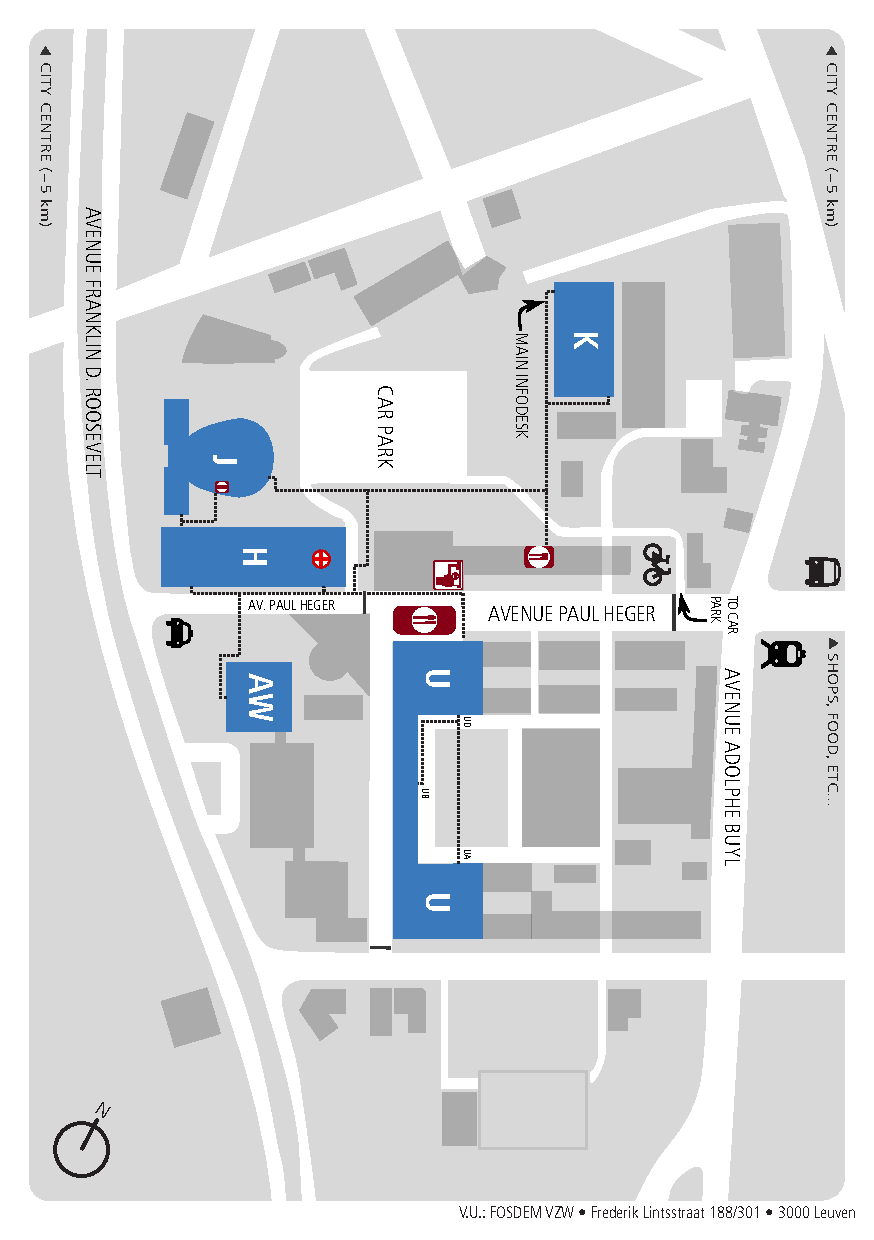
\includegraphics[width=\textwidth]{artwork/campusmap}

\end{document}
